\documentclass[a4paper]{article}

%Tutti gli usepackage vanno qui

\usepackage{geometry}
\usepackage[italian]{babel}
\usepackage[utf8]{inputenc}
\usepackage[T1]{fontenc}
\usepackage{tabularx}
\usepackage{longtable}
\usepackage{hyperref}
\usepackage{enumitem}
\hypersetup{
	colorlinks=true,
	linkcolor=black,
	filecolor=magenta,      
	urlcolor=blue,
}
% Numerazione figure 
\let\counterwithout\relax
\let\counterwithin\relax
\usepackage{chngcntr}

\counterwithin{table}{subsection}
\counterwithin{figure}{subsection}

\usepackage[bottom]{footmisc}
\usepackage{fancyhdr}
\usepackage{titlesec}
\setcounter{secnumdepth}{5}
\usepackage{amsmath, amssymb}
\usepackage{array}
\usepackage{graphicx}

%\usepackage{float}
\usepackage{layouts}
\usepackage{url}
\usepackage{comment}
\usepackage{float}
\usepackage{eurosym}


\usepackage{layouts}
\usepackage{float}
\usepackage{eurosym}

%Comandi di impaginazione uguale per tutti i documenti
\pagestyle{fancy}
\lhead{
\includegraphics[scale=0.07]{res/images/zeus_code_logo.png}}
%Titolo del documento
\rhead{\doctitle{}}
%\rfoot{\thepage}
\cfoot{Pagina \thepage\ di \pageref{LastPage}}
\setlength{\headheight}{35pt}
\setcounter{tocdepth}{5}
\setcounter{secnumdepth}{5}
\renewcommand{\footrulewidth}{0.4pt}

% multirow per tabelle
\usepackage{multirow}

% Permette tabelle su più pagine

%\usepackage{longtable}


% colore di sfondo per le celle
\usepackage[table]{xcolor}

%COMANDI TABELLE
\newcommand{\rowcolorhead}{\rowcolor[HTML]{56A5EC}} %intestazione 
\newcommand{\rowcolorlight}{\rowcolor[HTML]{FAFAFA}} %righe chiare/dispari
\newcommand{\rowcolordark}{\rowcolor[HTML]{E1F5FE}} %righe scure/pari
\newcommand{\colorhead}{\color[HTML]{FFFFFF}} %testo intestazione
\newcommand{\colorbody}{\color[HTML]{000000}} %testo righe
\newcommand{\tabitem}{~~\rlap{\textbullet}~~}

\newcommand{\glo}{$_{G}$}
\newcommand{\glosp}{$_{G}$ }

\definecolor{pari}{HTML}{E1F5FE}
\definecolor{dispari}{HTML}{FAFAFA}

%mettere il totale di pagine del doc a piè di pagina
\usepackage{lastpage}
%\fancypagestyle{plain} {
%	\fancyfoot[C]{Pagina \thepage\ di \pageref{LastPage}}}



%Lista dei comandi personalizzati
\newcommand{\doctitle}{Verbale esterno 2019-03-14}
\newcommand{\rev}{1.0.0}
\newcommand{\approv}{Irina Hornoiu}
\newcommand{\ver}{Riccardo Dario}
\newcommand{\red}{Marco Dalla Bà}
\newcommand{\stato}{Approvato}
\newcommand{\uso}{Esterno}
\newcommand{\describedoc}{Riassunto dell'incontro del gruppo \textit{Zeus Code} con GaiaGo tenutosi il 2019-03-11.}
\newcommand{\destinatari}{Zeus Code\\& GaiaGo\\& Prof. Tullio Vardanega\\& Prof. Riccardo Cardin}




\makeindex

\begin{document}

\thispagestyle{empty}
\begin{titlepage}
	\begin{center}
		
\includegraphics[scale = 0.3]{res/images/zeus_code_logo.png}\\
		\large \textbf{Zeus Code - Progetto "P2PCS"} \\
		\vfill
		\Huge \textbf{\doctitle}
		\vspace*{\fill}
		
		\vfill
		\large
		\begin{tabular}{r|l}
			\textbf{Versione} & \rev{} \\
	%		\textbf{Approvazione} & \approv{} \\
			\textbf{Redazione} & \red{} \\
			\textbf{Verifica} & \ver{} \\
			\textbf{Stato} & \stato{} \\
			\textbf{Uso} & \uso{} \\
			\textbf{Destinato a} & \parbox[t]{5cm}{Zeus Code
				\\Prof. Tullio Vardanega\\Prof. Riccardo Cardin}
		\end{tabular}
		\vfill
		\normalsize
		\textbf{Descrizione}\\
		\describedoc
		\vfill
		\small
		\texttt{zeuscode17@gmail.com}
	\end{center}
\end{titlepage}

\pagebreak
\section*{Tabelle delle modifiche}
\renewcommand{\arraystretch}{1.5}
\rowcolors{2}{pari}{dispari}
\begin{longtable}{ 
		>{\centering}p{0.09\textwidth} 
		>{\centering}p{0.13\textwidth}
		>{\centering}p{0.2\textwidth} 
		>{\centering}p{0.16\textwidth} 
		>{}p{0.2775\textwidth} }
	
	\rowcolorhead
	\textbf{\color{white}Versione} & 
	\textbf{\color{white}Data} & 
	\textbf{\color{white}Nominativo} & 
	\textbf{\color{white}Ruolo} &
	\centering \textbf{\color{white}Descrizione} 
	\tabularnewline  
	\endfirsthead
	\rowcolorhead
	\textbf{\color{white}Versione} & 
	\textbf{\color{white}Data} & 
	\textbf{\color{white}Nominativo} & 
	\textbf{\color{white}Ruolo} &
	\centering \textbf{\color{white}Descrizione} 
	\tabularnewline  
	\endhead
				1.0.0 & 2019-01-06 & Federico Bicciato & \textit{Responsabile 
				di Progetto} 
				& Approvazione del documento.
				
				\tabularnewline
				0.1.0 & 2019-01-05 & Paolo Pozzan & \textit{Verificatore} 
				& Modifica e revisione del documento.
				
				\tabularnewline
				0.0.1 & 2019-01-04 & Giacomo Greggio & \textit{Analista} 
				& Stesura del documento.
                                       
    
        
\end{longtable}



\counterwithin{table}{subsection}
\counterwithin{figure}{subsection}

\pagebreak

\tableofcontents

\pagebreak

\listoffigures

\pagebreak

\listoftables

\pagebreak

\counterwithin{table}{subsection}
\counterwithin{figure}{subsection}
\section{Introduzione}
\subsection{Scopo del documento}
Questo documento ha l'obiettivo di identificare e dettagliare la pianificazione del gruppo \textit{Zeus Code} relativa allo sviluppo del progetto \textit{P2PCS}. In particolare il documento tratta i seguenti argomenti:
\begin{itemize}
	\item analisi dei rischi;
	\item descrizione del modello di sviluppo adottato;
	\item ripartizione dei compiti tra i membri del gruppo;
	\item stima dei costi e delle risorse necessarie.
\end{itemize}
\subsection{Scopo del prodotto}
Lo scopo del prodotto è quello di sviluppare una piattaforma di Car Sharing Peer-to-Peer\glosp per l'applicazione Android\glosp sviluppata da \textit{GaiaGo}, un servizio di Car Sharing condominiale. L'obiettivo del capitolato\glosp consiste nel realizzare quest'applicazione sfruttando i meccanismi di gamification\glo; a questo fine
verrà utilizzato il framework\glosp \textit{Octalysis}\glo.
\subsection{Glossario}
Con l'obiettivo di evitare ridondanze e ambiguità di linguaggio, i termini tecnici e gli acronimi
utilizzati nei documenti verranno definiti e descritti riportandoli nel documento \textit{Glossario v1.0.0}.
I vocaboli riportati vengono indicati con una 'G' a pedice.
\subsection{Riferimenti}
\subsubsection{Normativi}
\begin{itemize}
	\item \textbf{Norme di Progetto}: \textit{Norme di Progetto v1.0.0};
	\item \textbf{Regolamento organigramma e specifica tecnico-economica}: \\
	\url{https://www.math.unipd.it/~tullio/IS-1/2018/Progetto/RO.html}.
\end{itemize}

\subsubsection{Informativi}
\begin{itemize}
	\item \textbf{Capitolato\glosp d'appalto C5 - \textit{P2PCS}: piattaforma di Peer-to-Peer\glosp car sharing}: \\
	\url{https://www.math.unipd.it/~tullio/IS-1/2018/Progetto/C5.pdf};
	\item \textbf{Slide L05 del corso Ingegneria del Software - Ciclo di vita 
		del software}:\\
	\url{https://www.math.unipd.it/~tullio/IS-1/2018/Dispense/L05.pdf};
	\item \textbf{Slide L06 del corso Ingegneria del Software - Gestione di 
	Progetto}: \\
	\url{https://www.math.unipd.it/~tullio/IS-1/2018/Dispense/L06.pdf};
	\item \textbf{Software Engineering - Ian Sommerville - 10$^{th}$ Edition, 
	2010}.
\end{itemize}

\hypertarget{scadenze}{\subsection{Scadenze}}
Il gruppo \textit{ZeusCode} si impegna a rispettare le seguenti scadenze per lo 
sviluppo del progetto \textit{P2PCS}:

\begin{itemize}
	\item \textbf{Revisione dei Requisiti}: 2019-04-19;
	\item \textbf{Revisione di Progettazione}: 2019-05-17;
	\item \textbf{Revisione di Qualifica}: 2019-06-17;
	\item \textbf{Revisione di Accettazione}: 2019-07-15.
\end{itemize}

\pagebreak
\section{Analisi dei rischi}

Durante lo sviluppo di un progetto avente grandi dimensioni è indispensabile prevenire 
futuri problemi tramite l'analisi dei rischi. Un'approfondita valutazione dei rischi permette la prevenzione e l'arginamento di problemi che intaccherebbero la buona riuscita del prodotto finale.\\
Sarà adottata la seguente procedura durante lo sviluppo del progetto:

\begin{itemize}
	\item \textbf{Individuazione dei rischi}: fase di identificazione dei fattori di rischio che possono interferire con l'avanzamento regolare del progetto;
	\item \textbf{Analisi dei rischi}: fase di studio dei rischi individuati, procede con l'assegnazione di una probabilità e di una pericolosità individuali;
	\item \textbf{Pianificazione di controllo}: fase in cui viene indicato come affrontare e prevenire
	i problemi derivati dai fattori di rischio;
	\item \textbf{Monitoraggio dei rischi}: processo ciclico al fine di evitare gli errori arginando i 
	fattori di rischio.
\end{itemize}
Ogni problema deriva da rischi diversi, ogni rischio viene rappresentato da uno dei seguenti codici:

\begin{itemize}
	\item \textbf{RT}: Rischi Tecnologici;
	\item \textbf{RO}: Rischi Organizzativi;
	\item \textbf{RI}: Rischi Interpersonali.
	\item \textbf{RR}: Rischi dei Requisiti.
\end{itemize}

\counterwithin{table}{section}
\renewcommand{\arraystretch}{1.5}
\rowcolors{2}{dispari}{pari}
	\arrayrulecolor{white}
	\begin{longtable}{ 
			>{\centering}p{0.17\textwidth} 
			>{\raggedright}p{0.28\textwidth}
			>{\raggedright}p{0.29\textwidth} 
			>{\centering}p{0.15\textwidth}
		}

	
	\caption{Tabella dei Rischi di Progetto}\\
	\rowcolorhead
	\colorhead\textbf{Codice \\ Nome} & \centering\colorhead\textbf{Descrizione} & 
	\centering\colorhead\textbf{Rilevamento} & 
	\colorhead\textbf{Grado di rischio} 
	\tabularnewline
	\endfirsthead
	\rowcolor{white}\caption[]{(continua)}\\
	\rowcolorhead
	\colorhead\textbf{Nome \\ Codice} & \centering\colorhead\textbf{Descrizione} & 
	\centering\colorhead\textbf{Rilevamento} & 
	\colorhead\textbf{Grado di rischio} 
	\tabularnewline
	\endhead
	
	%RT1---------------------------------------------------------
	 \textbf{RT1} \\ Inesperienza Tecnologica & 
	 Alcune delle tecnologie adottate sono nuove ad alcuni membri
	 del team, pertanto è possibile incorrere in problemi durante lo svolgimento delle attività che le coinvolgono. &
	 Ciascun membro del gruppo è incaricato di far presente al \textit{Responsabile} 
	 le proprie lacune e difficoltà. &
	 Occorrenza: \textbf{Alta} \\
	 Pericolosità: \textbf{Alta} 
	 \tabularnewline
	\rowcolorlight \multicolumn{1}{p{0.17\textwidth}}{\centering{Piano di contingenza}}& 
	 \multicolumn{3}{p{0.7775\textwidth}}{Verranno suddivisi i membri in piccoli gruppi, in modo da
	 	affrontare insieme i compiti più onerosi. }
	 \tabularnewline 
	\pagebreak
	
		%RT2---------------------------------------------------------
	\textbf{RT2} \\ Hardware personale & 
	Esiste la possbilità che i supporti hardware utilizzati da uno o più membri del gruppo siano soggetti a guasti e di conseguenza ci sia una perdita locale dei dati. &
	Ciascun membro del gruppo è responsabile del proprio materiale e dovrà far fronte ad eventuali guasti tramite l'utilizzo di software di versionamento. &
	Occorrenza: \textbf{Basso} \\
	Pericolosità: \textbf{Media} 
	\tabularnewline
	\rowcolorlight \multicolumn{1}{p{0.17\textwidth}}{\centering{Piano di contingenza}}& 
	\multicolumn{3}{p{0.7775\textwidth}}{In caso di perdita definitiva di dati i membri del gruppo si adoperano alla loro immediata riformazione. }
	\tabularnewline  	
	 	
	 %RO1---------------------------------------------------------
	\rowcolordark \textbf{RO1} \\ Tempistiche  &
	Essendo un metodo di lavoro nuovo per il team, non sempre il calcolo preventivo in termini di tempo 
	per svolgere un'attività sarà rispettato.&
	Ogni task ha la propria data di inizio e di fine, ogni variazione sulla data di scadenza dovrà
	essere comunicata e seguita da una descrizione.&	
	Occorrenza: \textbf{Alta} \\
	Pericolosità: \textbf{Alta}
	\tabularnewline
	\rowcolordark\multicolumn{1}{p{0.17\textwidth}}{\centering{Piano di contingenza}}& 
	\multicolumn{3}{p{0.7775\textwidth}}{All'insorgere di tali problematiche, 
	il \textit{Responsabile} gestirà le risorse in modo da ridurre i ritardi nel modo
	più efficiente possibile.}
	\tabularnewline	
	
	%R02------------------------------------------------------------
	\rowcolorlight	\textbf{RO2} \\ Calcolo dei \\costi &
	A causa dell'inesperienza del team in ambito lavorativo, la possibilità di incorrere in errori
	di valutazione è plausibile. &
	Il \textit{Responsabile} dispone delle schedule\glosp di lavoro di ogni membro del gruppo così da verificare 
	l'effettivo monte ore.&
	Occorrenza: \textbf{Media} \\
	Pericolosità: \textbf{Alta}
	\tabularnewline
	\rowcolorlight\multicolumn{1}{p{0.17\textwidth}}{\centering{Piano di contingenza}}& 
	\multicolumn{3}{p{0.7775\textwidth}}{Verrà rivalutata una differente distribuzione del lavoro in caso di costi eccessivi.}
	\tabularnewline	
	
	%R03------------------------------------------------------------
	\rowcolordark\textbf{RO3} \\ Impegni Accademici e Personali& 
	Si possono creare dei momenti in cui uno o più membri del gruppo non siano disponibili
	a causa di impegni scolastici o personali. &
	Viene predisposto un calendario condiviso accessibile a tutti i membri del gruppo, in modo da indicare
	le date e gli orari disponibili di ognuno.&
	Occorrenza: \textbf{Alta} \\
	Pericolosità: \textbf{Bassa}
	\tabularnewline
	\rowcolordark\multicolumn{1}{p{0.17\textwidth}}{\centering{Piano di contingenza}}& 
	\multicolumn{3}{p{0.7775\textwidth}}{ Il carico di lavoro sarà distribuito, nel modo più efficiente possibile, 
		in base agli impegni dei membri durante tutto l'arco di sviluppo.}
	\tabularnewline	
	
	%R05------------------------------------------------------------
	\rowcolordark
	\textbf{RO4} \\ Ritardi  &
	Le problematiche sopracitate possono causare ritardi.&
	Ogni componente segnalerà tempestivamente l'eventuale ritardo.&
	Occorrenza: \textbf{Media} \\
	Pericolosità: \textbf{Bassa}
	\tabularnewline
	\rowcolordark\multicolumn{1}{p{0.17\textwidth}}{\centering{Piano di contingenza}}& 
	\multicolumn{3}{p{0.7775\textwidth}}{ Il \textit{Responsabile}, se 
	necessario, 
	riassegnerà le risorse al fine di evitare rallentamenti.}
	\tabularnewline	
	
	%RI1------------------------------------------------------------
	\rowcolorlight
	\textbf{RI1} \\ Comunicazione Interna  & 
	Uno o più membri del gruppo possono risultare irreperibili. &
	Tutti i membri sono tenuti a segnalare eventuali periodi di irraggiungibilità. &
	Occorrenza: \textbf{Bassa} \\
	Pericolosità: \textbf{Alta}
	\tabularnewline
	\rowcolorlight\multicolumn{1}{p{0.17\textwidth}}{\centering{Piano di contingenza}}& 
	\multicolumn{3}{p{0.7775\textwidth}}{Solitamente questo rischio può essere causato da un emergenza e i soliti canali di comunicazione
		potrebbero essere insufficienti.
		Per ovviare al precedente problema vengono organizzati incontri settimanali in concordanza tra tutti membri.}
	\tabularnewline	
	
	%RI2------------------------------------------------------------
	\rowcolordark
	\textbf{RI2} \\ Comunicazione Esterna &
	Il proponente, essendo una realtà imprenditoriale, non sempre è disposto alla comunicazione immediata con il gruppo.
	Potrebbero verificarsi casi di impossibilità di comunicazione per vari periodi di tempo. &
	Verranno definite delle date per le riunioni con largo anticipo in comune accordo con il proponente.&
	Occorrenza: \textbf{Bassa} \\
	Pericolosità: \textbf{Media}
	\tabularnewline
	\rowcolordark\multicolumn{1}{p{0.17\textwidth}}{\centering{Piano di contingenza}}& 
	\multicolumn{3}{p{0.7775\textwidth}}{In caso di ritardi il gruppo procederà seguendo i canoni imposti dal capitolato\glo,
		in attesa di una futura relazione col proponente.}
	\tabularnewline	
	
	%RI3------------------------------------------------------------
	\rowcolorlight
	\textbf{RI3} \\ Contrasti interni &
	Essendo un gruppo di persone alle prime armi è possibile incorrere in contrasti e tensioni tra i membri. &
	Si fa affidamento sulla maturità dei vari membri, i quali cercheranno di mantenere un clima di reciproco rispetto ed 
	eviteranno eventuali contrasti. &
	Occorrenza: \textbf{Bassa} \\
	Pericolosità: \textbf{Alta}
	\tabularnewline
	\rowcolorlight\multicolumn{1}{p{0.17\textwidth}}{\centering{Piano di contingenza}}& 
	\multicolumn{3}{p{0.7775\textwidth}}{In caso di controversie riguardanti aspetti del progetto sarà compito del \textit{Responsabile} 
		decidere tra le varie alternative proposte.}
	\tabularnewline	
	
	%RR1------------------------------------------------------------
	\rowcolorlight
	\textbf{RR1} \\ Variazione dei requisiti &
	È possibile che alcuni requisiti individuati dagli analisti siano errati o che non coincidano con quanto richiesto dal proponente. Ciò prevede una rimozione e/o correzione di eventuali mancanze &
	Si argina questo rischio tramite il continuo confronto col proponente sia in via telematica che tramite incontri in sede universitaria. &
	Occorrenza: \textbf{Bassa} \\
	Pericolosità: \textbf{Alta}
	\tabularnewline
	\rowcolorlight\multicolumn{1}{p{0.17\textwidth}}{\centering{Piano di contingenza}}& 
	\multicolumn{3}{p{0.7775\textwidth}}{Nel caso alcuni requisiti risultino errati sarà necessario provvedere alla loro immediata rimozione o modifica.}
	\tabularnewline	
		
	\end{longtable}
\counterwithin{table}{subsection}	
\renewcommand{\arraystretch}{1}


\pagebreak
\section{Modello di sviluppo}
La scelta del modello di sviluppo\glosp è una delle realtà fondamentali per la realizzazione di un progetto software.
Avendo una visione abbastanza chiara dell'intero progetto e, allo stesso tempo, una limitata conoscenza dei requisiti specifici, si è scelto di seguire il \textbf{modello incrementale}.

\begin{figure}[H]
	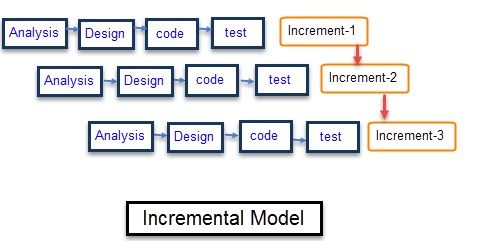
\includegraphics[width=0.99\linewidth]{res/images/incremental_model.jpg}
	\caption{Modello di sviluppo incrementale}
\end{figure}

\subsection{Modello incrementale}
Il modello di sviluppo incrementale permette la suddivisione del progetto in più sottoinsiemi,
ognuno dei quali incorpora una funzionalità diversa che, se necessario, verrà migliorata ad ogni incremento.  \\
Ad ogni incremento del sistema è consentita la modifica, aggiunta ed eliminazione di requisiti in base alle esigenze progettuali; 
è necessario un colloquio diretto con il proponente per approvare tali cambiamenti. \\
Utilizzando questo modello di sviluppo il versionamento del sistema è reso semplice e intuitivo, in quanto ogni modifica è facilmente tracciabile da un incremento all'altro e se ne possono valutare direttamente i difetti o benefici.\\
I vantaggi predisposti dal modello incrementale sono i seguenti:
\begin{itemize}
	\item gli incrementi sono disposti in base alle funzionalità con priorità decrescente, partendo da quelle con priorità e impatto maggiori
	così da avere subito un riscontro diretto;
	\item ogni incremento genera un risultato che può essere valutato dal proponente, approvandone i benefici o evidenziandone i difetti;
	\item rende sempre disponibile una recente baseline\glosp per una eventuale rivalutazione, senza dover ripercorrere tutti i passi effettuati fino ad ora dall'inizio dello sviluppo;
	\item tutti gli errori sono limitati al singolo incremento;
	\item le modifiche e le correzioni sono molto economiche in quanto di facile reperibilità;
	\item le fasi di test sono mirate al corrente incremento, quindi più efficienti.
\end{itemize}
Sono presenti anche degli aspetti negativi per quanto riguarda il modello incrementale. La suddivisione di un singolo problema in più parti, dove almeno una di esse richiede una modifica, comporta una nuova elaborazione anche delle altre parti che non sono direttamente coinvolte, ciò aumenta in modo considerevole i tempi di sviluppo.
I problemi potrebbero derivare anche dall'architettura del sistema, la quale potrebbe non riuscire a soddisfare tutti i requisiti raccolti in anticipo per l'intero ciclo di vita del software.




\pagebreak
\section{Pianificazione}
La pianificazione del lavoro all'interno del gruppo \textit{Zeus Code} segue i canoni dettati nella sezione \hyperlink{scadenze}{sottosezione 1.5}, la pianificazione di progetto viene suddivisa nelle seguenti fasi:
\begin{enumerate}
	\item \textbf{Analisi};
	\item \textbf{Consolidamento dei requisiti};
	\item \textbf{Progettazione architetturale};
	\item \textbf{Progettazione di dettaglio e codifica};
	\item \textbf{Validazione e collaudo}.
\end{enumerate}
Ogni fase consiste in un insieme di attività aventi una data di inizio e una di fine, il tutto viene riportato nei diagrammi di Gantt\glo. Viene fissata come data di scadenza il giorno di consegna dei materiali prodotti dalle attività. 
\subsection{Analisi}
\textit{Periodo: dal 2019-01-03 al 2019-04-19}\\
L'inizio di questa fase coincide con la formazione dei gruppi del secondo lotto e la fine corrisponde con la data ultima per la consegna dei documenti relativi alla Revisione dei Requisiti.
Questa fase è stata scomposta nelle seguenti sotto attività:
\begin{itemize}
	\item \textbf{Individuazione degli strumenti}: vengono scelti gli strumenti che saranno impiegati per la parte riguardante le comunicazioni tra membri, vengono inoltre definiti i programmi utili alla scrittura di file \LaTeX; 
	\item \textbf{Norme di Progetto}: utilizzando gli strumenti sopra indicati si stende il documento \textit{Norme di progetto v1.0.0} indipendente dal capitolato scelto. Il documento Norme di Progetto viene redatto dall'\textit{Amministratore} per conto del \textit{Responsabile di progetto};
	\item \textbf{Studio di fattibilità}: è compito degli \textit{Analisti} effettuare uno studio dei vari capitolati per evidenziarne pregi e difetti e scegliere il capitolato da sviluppare. Fase bloccante per l'Analisi dei Requisiti;
	\item \textbf{Analisi dei Requisiti}: questa attività è volta alla produzione del documento \textit{Analisi dei requisiti v1.0.0}, questo file è in continua fase di miglioramento fino alla data di consegna;
	\item \textbf{Piano di Progetto}: il \textit{Responsabile} analizza le singole attività e le loro date di scadenza in modo da gestire le risorse necessarie al loro completamento, viene redatto il documento \textit{Piano di progetto v1.0.0};
	\item \textbf{Piano di Qualifica}: attività volta alla redazione del file \textit{Piano di qualifica v1.0.0}, il quale individua le metodologie implicate nel garantire la qualità del prodotto; 
	\item \textbf{Glossario}: documento volto a racchiudere tutti termini che possono risultare ambigui o che semplicemente necessitano di una descrizione appropriata onde evitare incomprensioni.
	\item \textbf{Lettera di presentazione}: questa attività consiste nella redazione della Lettera di Presentazione necessaria  per  la  presentazione del gruppo \textit{Zeus Code} come fornitore.
\end{itemize}
%DA METTERE GANTT
%\begin{figure}[H]
%	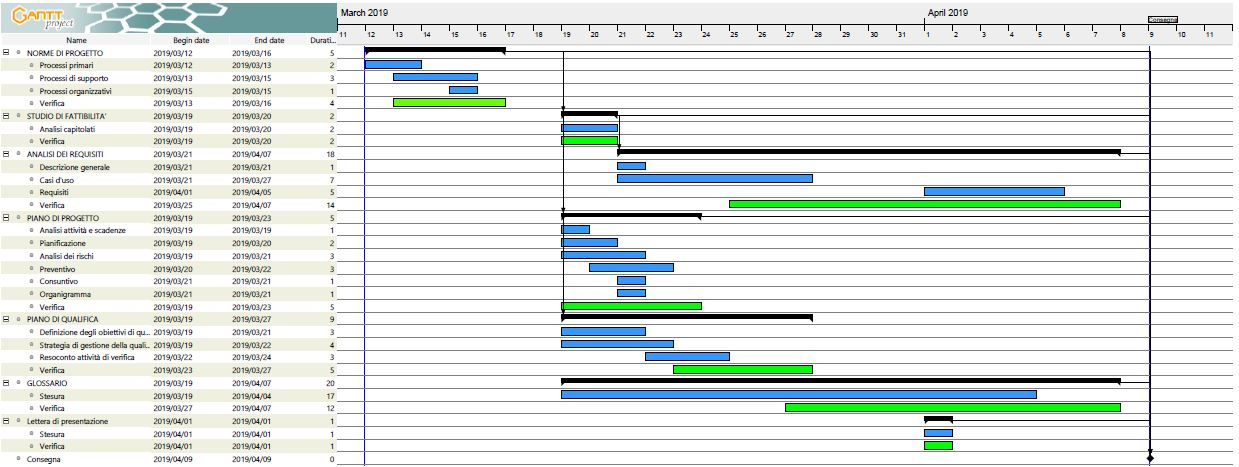
\includegraphics[width=0.99\linewidth]{res/images/gantt_analisi.jpg}
%	\caption{Diagramma di Gantt della fase di Analisi}
%\end{figure}

\subsection{Consolidamento dei requisiti}
\textit{Periodo: dal 2019-03-28 al 2019-04-19} \\
Questa fase ha inizio dopo l'attività di analisi e termina con la consegna dei documenti per la Revisione dei Requisiti. Le attività 
di questa fase sono:
\begin{itemize}
	\item \textbf{Consolidamento}: vengono migliorati i requisiti ottenuti nella fase di analisi;
	\item \textbf{Preparazione alla presentazione}: viene pianificata la scaletta da seguire per la presentazione del 2019-04-19;
	\item \textbf{Incremento e Verifica}: vengono rivalutati singolarmente tutti i file e in caso saranno soggetti a miglioramenti e modifiche;
	\item \textbf{Approfondimento personale}: i membri del team dedicheranno un monte ore, da loro predisposto, per studiare le nuove tecnologie richieste dal capitolato\glo.Questa attività verrà svolta in modo autonomo e quindi non è riportata nel seguente diagramma di Gantt.%~\ref{fig:gantt_con}.
\end{itemize}
%
%\begin{figure}[H]
%	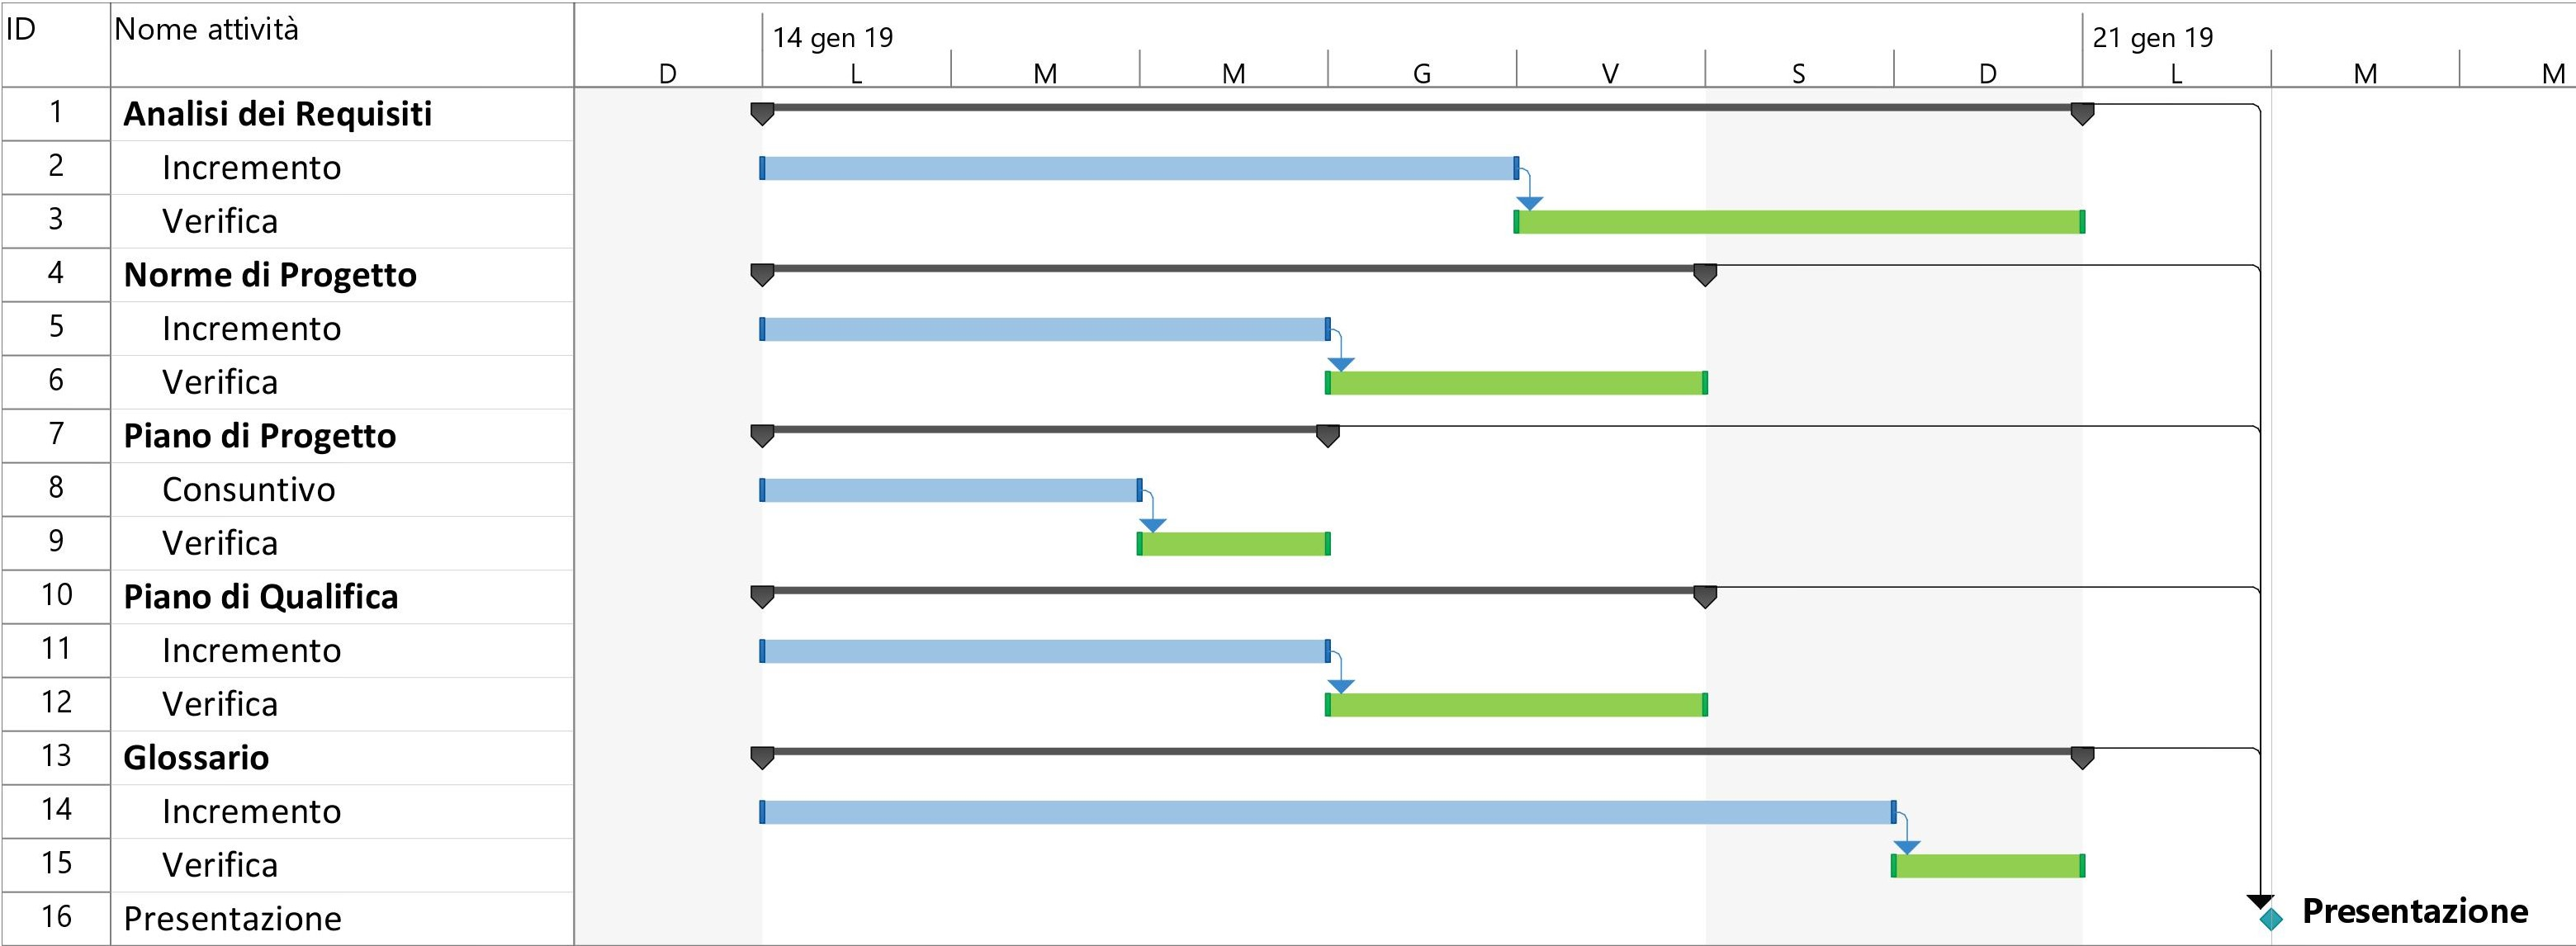
\includegraphics[width=0.99\linewidth]{res/images/gantt_cons.jpg}
%	\caption{Diagramma di Gantt della fase di Consolidamento dei requisiti}
%	\label{fig:gantt_con}
%\end{figure}

%-----------------Sottosezione Progettazione Architetturale---------------------
\subsection{Progettazione architetturale}
\textit{Periodo: dal 2019-04-19 al 2019-05-17} \\
Il periodo di Progettazione architetturale inizia il giorno successivo alla presentazione per la Revisione dei Requisiti e si conclude con la data di consegna Revisione di 
Progettazione. In questo periodo le attività principali sono:
\begin{itemize}
	\item \textbf{Technology Baseline}: redazione del documento \textit{Specifica Tecnica v1.0.0} per la descrizione delle scelte progettuali ad alto livello del prodotto finale.
	Il documento definisce i design pattern\glosp che verranno utilizzati,l'architettura del prodotto e il tracciamento dei requisiti.\\
	Infine viene codificato il \textbf{Proof of Concept}\glosp il 
	quale viene presentato o condiviso tramite repository al committente e 
	proponente in una data da definirsi;
	\item \textbf{Incremento e Verifica}: se necessario vengono migliorati i 
	documenti prodotti nelle fasi precedenti.
\end{itemize}

%\begin{figure}[H]
%	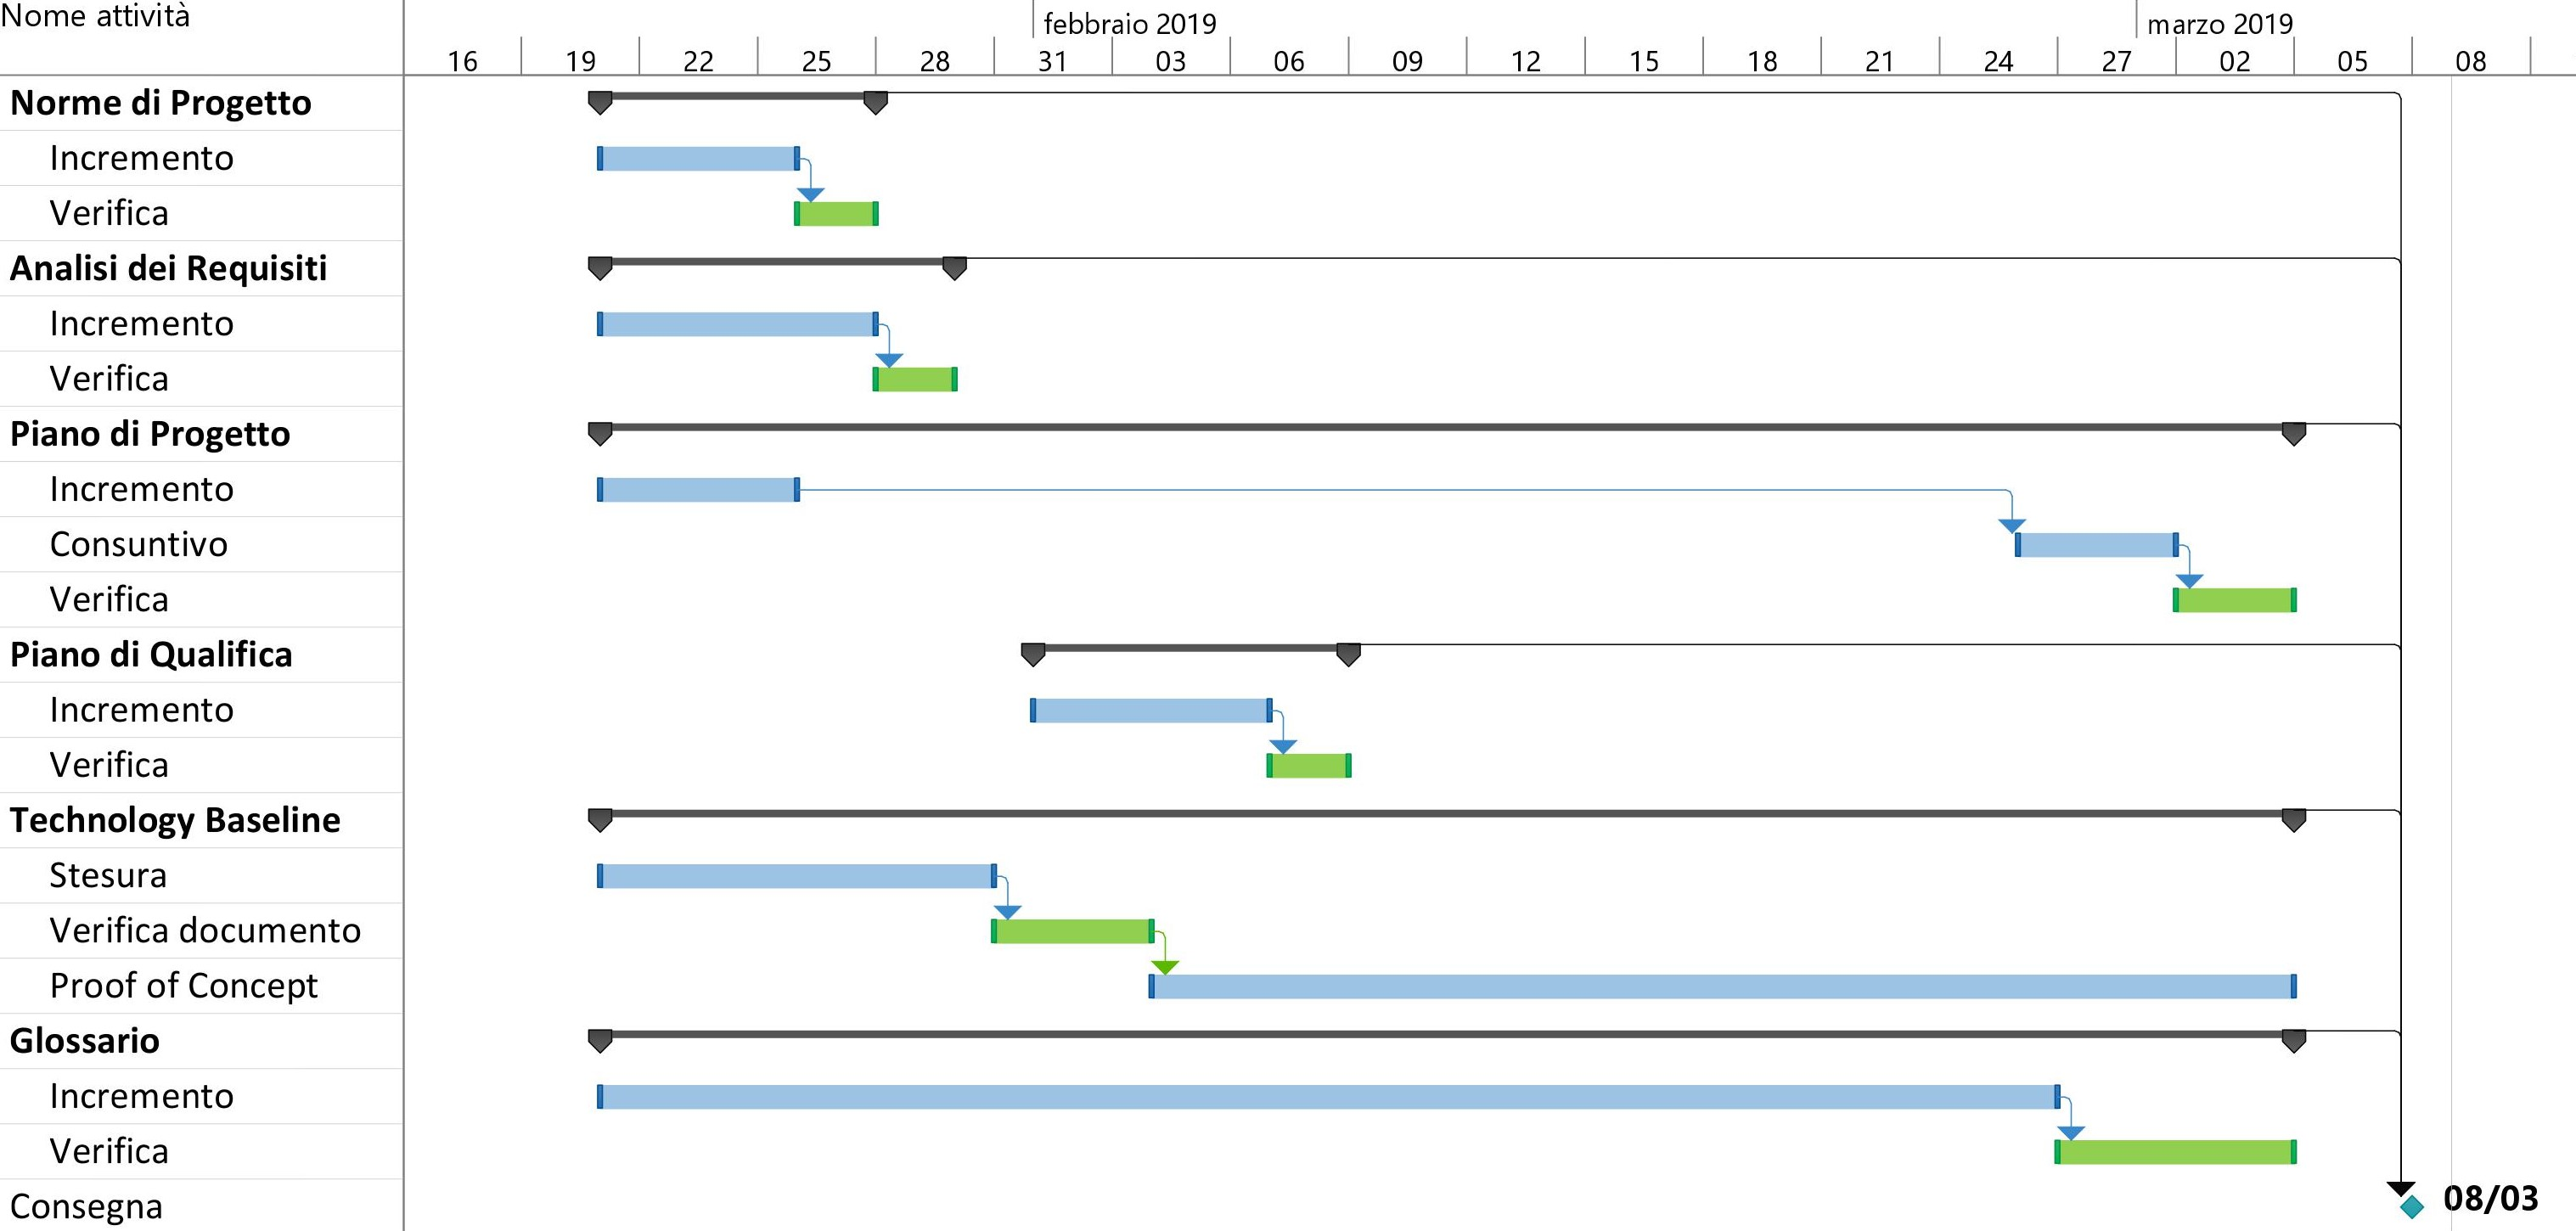
\includegraphics[width=0.99\linewidth]{res/images/gantt_pa.jpg}
%	\caption{Diagramma di Gantt della fase di Progettazione architetturale}
%\end{figure}


%-------------------Sottosezione Progettazione di Dettaglio---------------------
\subsection{Progettazione di dettaglio e codifica}
\textit{Periodo: dal 2019-05-17 al 2019-06-17}
Il periodo di Progettazione di dettaglio e codifica inizia il giorno dopo la Revisione di progettazione e termina con la data di consegna dei documenti 
in vista della Revisione di Qualifica. Le attività di questa fase sono:
\begin{itemize}
	\item \textbf{Product Baseline}: a seguito della \textit{Technology 
	Baseline} l'architettura in essa individuata viene scomposta nelle sue unità, ciò permettere di iniziare con la fase di progettazione di basso livello. Segue la redazione del documento Definizione di Prodotto;
	\item \textbf{Codifica}: questa attività consiste nella scrittura del 
	codice e della sua verifica con modalità e strumenti definiti nel 
	\textit{Piano di Qualifica v1.0.0};
	\item \textbf{Manuale Utente}: attività volta alla redazione del documento Manuale Utente, contenente le indicazioni per l'utilizzo del prodotto;
	\item \textbf{Incremento e Verifica}: se necessario vengono migliorati i 
	documenti prodotti nelle fasi precedenti.
\end{itemize}

%\begin{figure}[H]
%	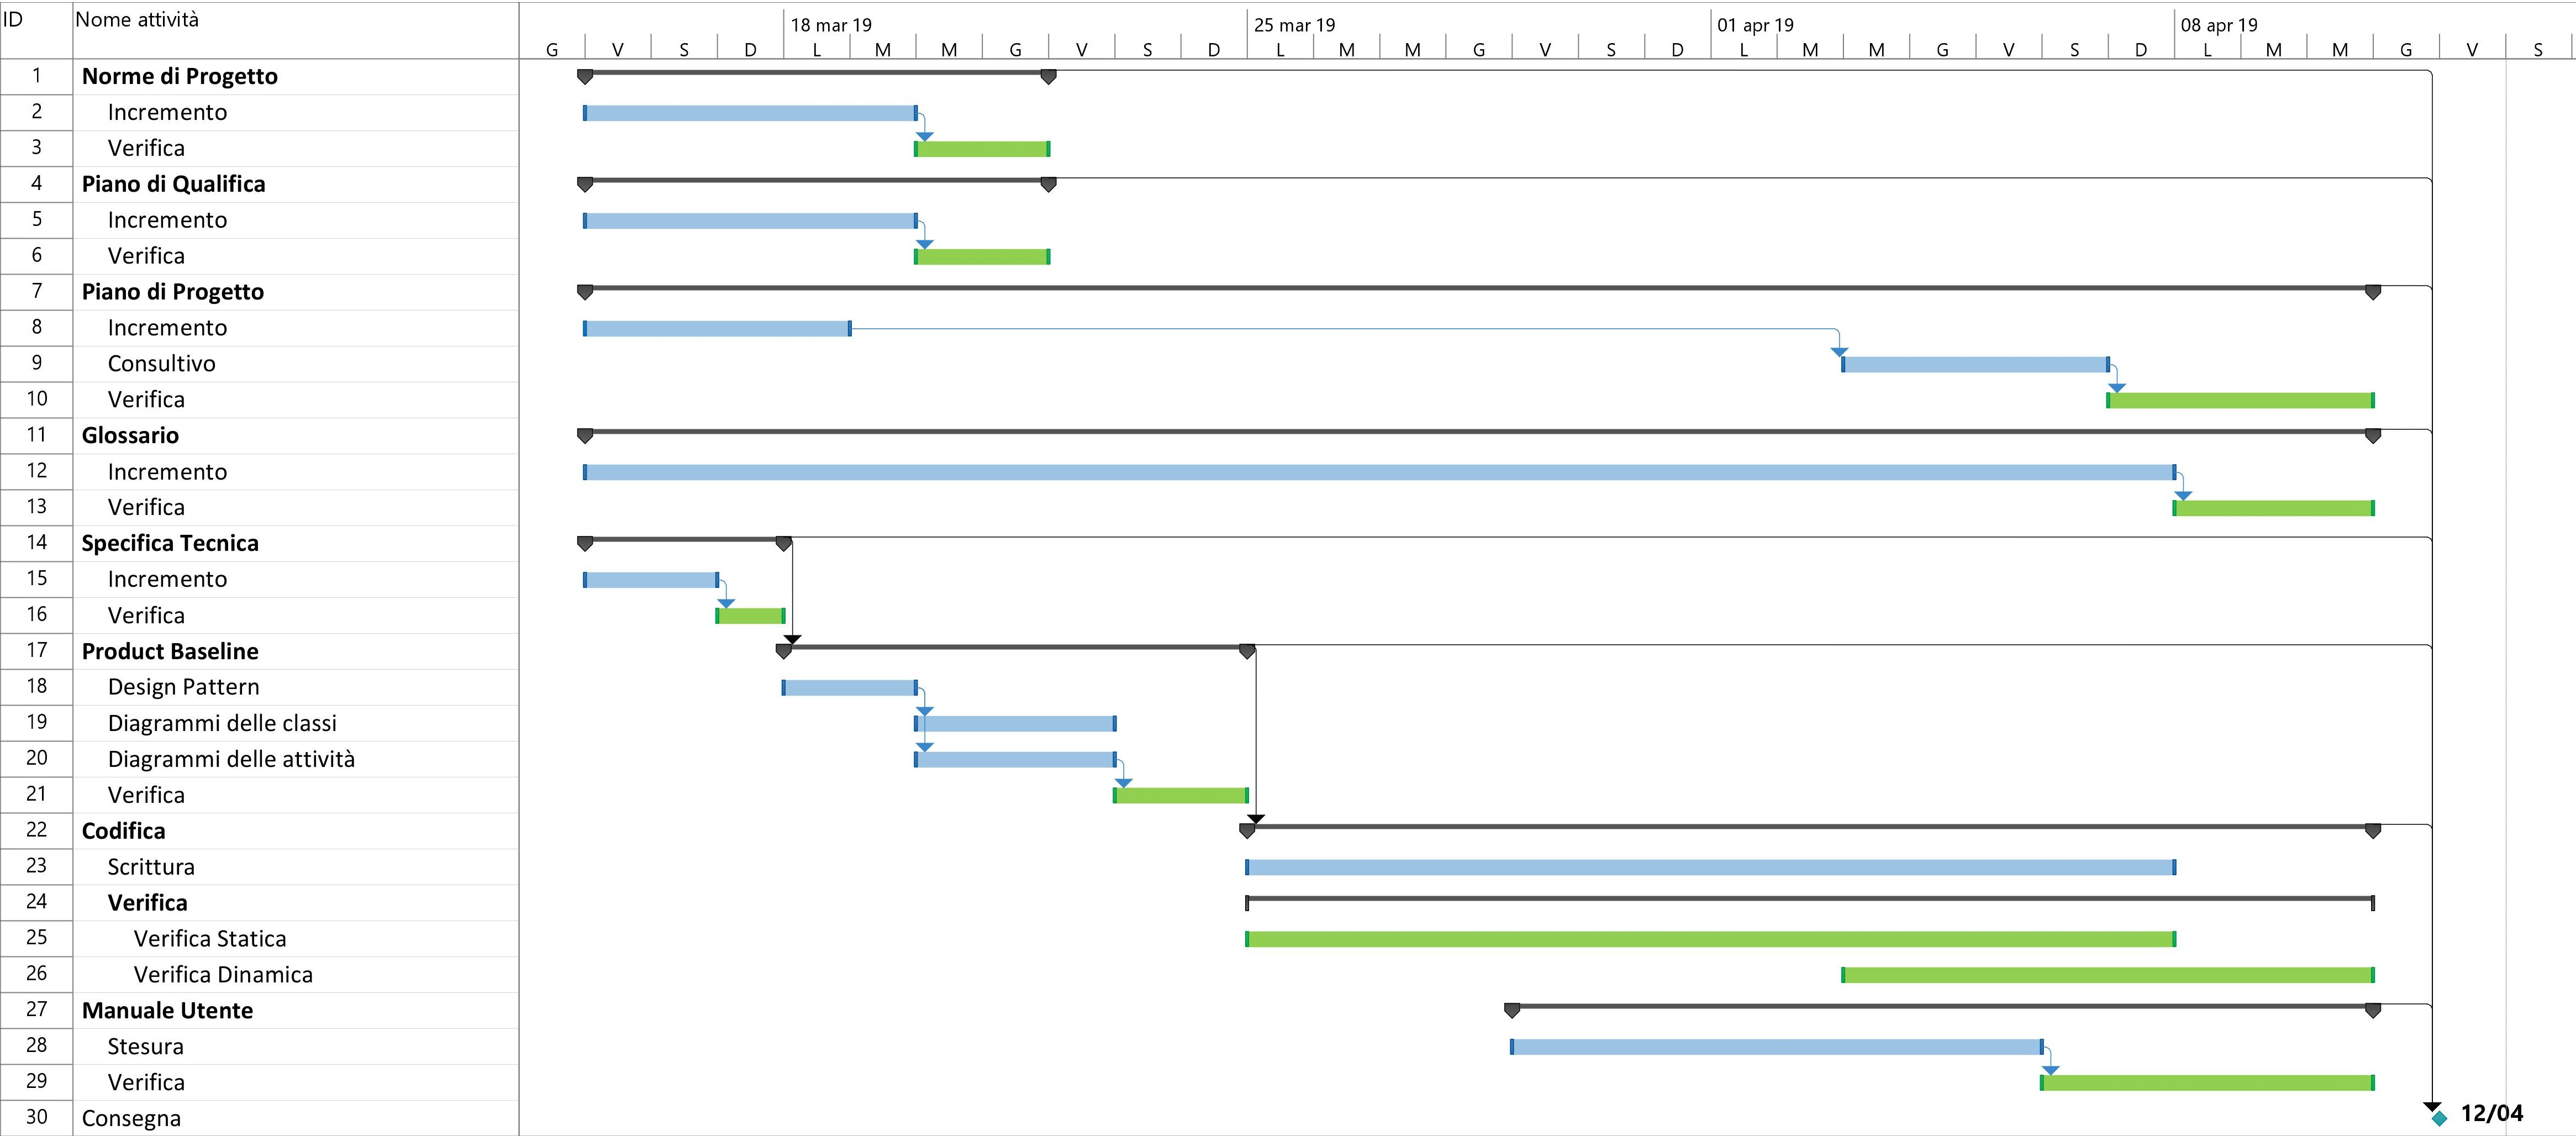
\includegraphics[width=0.99\linewidth]{res/images/gantt_pd.jpg}
%	\caption{Diagramma di Gantt della fase di Progettazione di dettaglio e codifica}
%\end{figure}
%\pagebreak


\subsection{Validazione e collaudo}
\textit{Periodo: dal 2019-04-12 al 2019-05-17 } \\
Il periodo di Validazione e collaudo inizia il giorno successivo alla data di consegna dei documenti per la 
Revisione di Qualifica e si conclude con la data di consegna in vista della Revisione di Accettazione. In questo periodo le attività principali sono:
\begin{itemize}
	\item \textbf{Validazione e Collaudo}: verranno eseguiti test mirati su possibili punti critici del prodotto finito e test generali per valutarne l'effettiva qualità;
	\item \textbf{Manuale Sviluppatore}: viene redatto il documento \textit{Manuale Sviluppatore} atto a fornire tutte le informazioni necessarie al mantenimento, manutenzione e ampliamento del prodotto finale;
	\item \textbf{Incremento e Verifica}: se necessario vengono migliorati i 
	documenti prodotti nelle fasi precedenti.
\end{itemize}
%\begin{figure}[H]
%	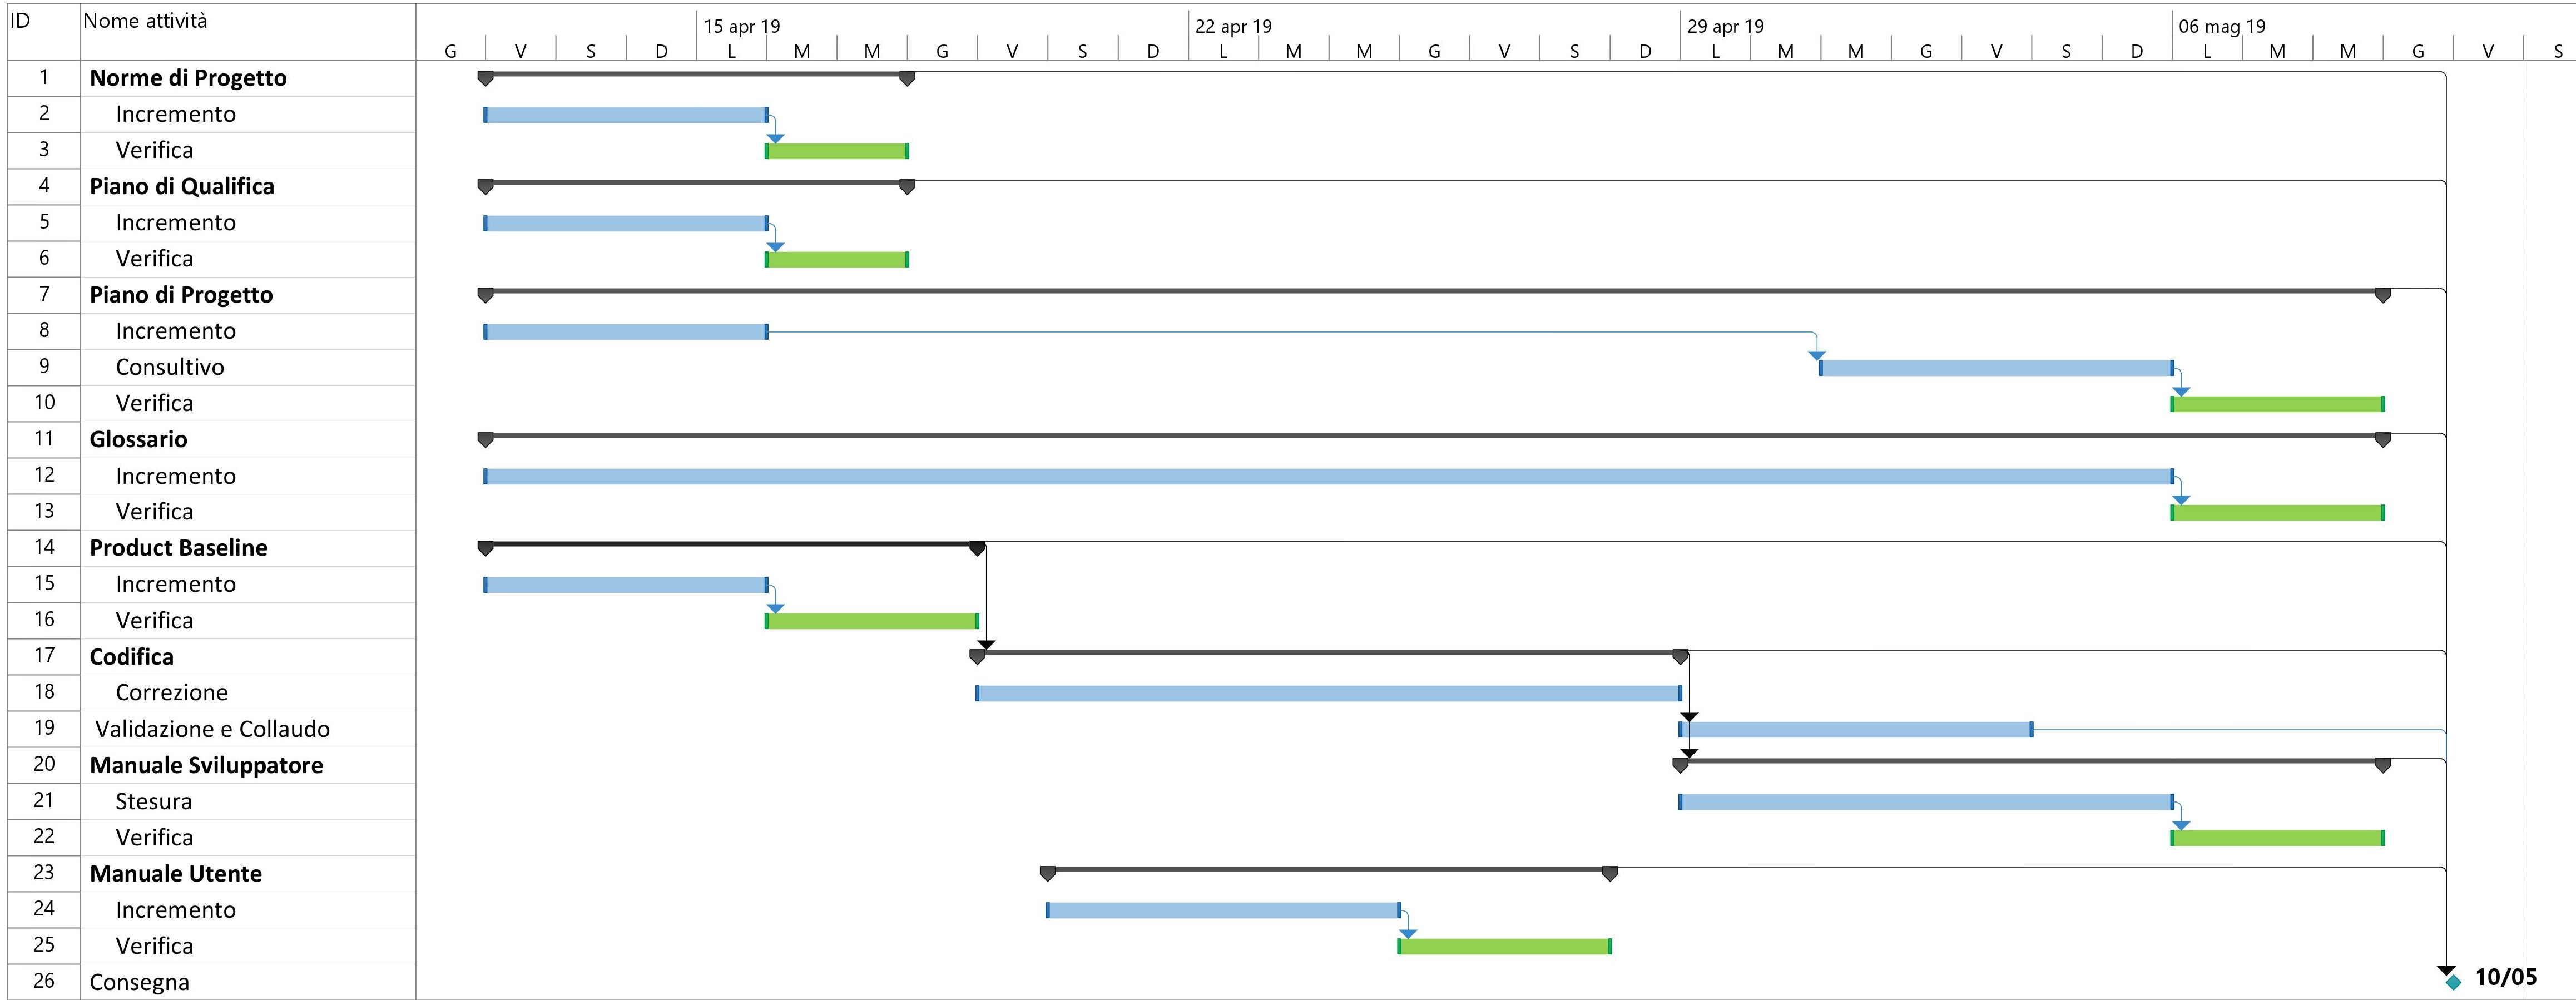
\includegraphics[width=0.99\linewidth]{res/images/gantt_val.jpg}
%	\caption{Diagramma di Gantt della fase di Validazione e collaudo}
%\end{figure}

\pagebreak
\section{Preventivo}
Per facilitare la lettura delle seguenti tabelle, vengono utilizzate delle sigle 
per identificare i ruoli:
\begin{itemize}
\item \textbf{Re:} \textit{Responsabile};
\item \textbf{Ad:} \textit{Amministratore};
\item \textbf{An:} \textit{Analista};
\item \textbf{Pt:} \textit{Progettista};
\item \textbf{Pr:} \textit{Programmatore};
\item \textbf{Ve:} \textit{Verificatore}.
\end{itemize}
\noindent
Inoltre, se le ore ricoperte in un determinato ruolo fossero nulle, la cella 
presenterà il simbolo \textbf{-} per indicarne l'assenza. 

\subsection{Fase di Analisi}
\subsubsection{Prospetto orario}
In questa fase, ogni componente del gruppo rivestirà i seguenti ruoli:
\begin{table}[H]
				\centering\renewcommand{\arraystretch}{1.5}
				\caption{Distribuzione delle ore nel periodo di Analisi}
				\vspace{0.2cm}
                \begin{tabular}{c c c c c c c c}
                               
                \rowcolorhead
                 {\colorhead \textbf{Nominativo}} &
                 {\colorhead \textbf{Re}} & 
                 {\colorhead \textbf{Am}} & 
                 {\colorhead\textbf{An}} & 
                 {\colorhead \textbf{Pt}} & 
                 {\colorhead\textbf{Pr}} & 
                 {\colorhead \textbf{Ve}} & 
                 {\colorhead \textbf{Ore totali} }\\
				
                \rowcolorlight
                 {\colorbody Federico Bicciato} & {\colorbody 5} & 
                 {\colorbody 5} & {\colorbody 10} & {\colorbody 5} & 
                 {\colorbody -} & {\colorbody 10} & {\colorbody 35} 
				\\
				
				\rowcolordark
                 {\colorbody Mattia Bolzonella} & {\colorbody -} & 
                 {\colorbody 8} & {\colorbody 17} & {\colorbody -} & 
                 {\colorbody -} & {\colorbody 10} & {\colorbody 35} 
				\\	
				
				\rowcolorlight
                 {\colorbody Francesco Donè} & {\colorbody 5} & 
                 {\colorbody -} & {\colorbody 17} & {\colorbody -} & 
                 {\colorbody -} & {\colorbody 13} & {\colorbody 35} 
				\\
				              
                \rowcolordark
                 {\colorbody Sara Feltrin} & {\colorbody 8} & 
                 {\colorbody 8} & {\colorbody 10} & {\colorbody 4} & 
                 {\colorbody -} & {\colorbody 5} & {\colorbody 35} 
				\\
				
				\rowcolorlight
                 {\colorbody Giacomo Greggio} & {\colorbody -} & 
                 {\colorbody 13} & {\colorbody 7} & {\colorbody -} & 
                 {\colorbody -} & {\colorbody 15} & {\colorbody 35} 
				\\
				
				\rowcolordark
                 {\colorbody Samuele Giuliano Piazzetta} & {\colorbody -} & 
                 {\colorbody -} & {\colorbody 15} & {\colorbody 5} & 
                 {\colorbody -} & {\colorbody 15} & {\colorbody 35} 
				\\	
				
				\rowcolorlight
                 {\colorbody Paolo Pozzan} & {\colorbody 6} & 
                 {\colorbody 10} & {\colorbody 8} & {\colorbody 5} & 
                 {\colorbody -} & {\colorbody 6} & {\colorbody 35} 
				\\
				
				\rowcolordark
                 {\colorbody Matteo Santinon} & {\colorbody 7} & 
                 {\colorbody -} & {\colorbody 12} & {\colorbody -} & 
                 {\colorbody -} & {\colorbody 16} & {\colorbody 35} 
				\\
				
				\rowcolorlight
                 {\colorbody \textbf{Ore totali ruolo}} & {\colorbody 31} & 
                 {\colorbody 44} & {\colorbody 96} & {\colorbody 19} & 
                 {\colorbody -} & {\colorbody 90} & {\colorbody 280} 
				\\
                

                \end{tabular}
               
\end{table}
\pagebreak
I dati ottenuti si possono riassumere nel seguente istogramma:
\begin{figure}[H] 
			\centering 
	%			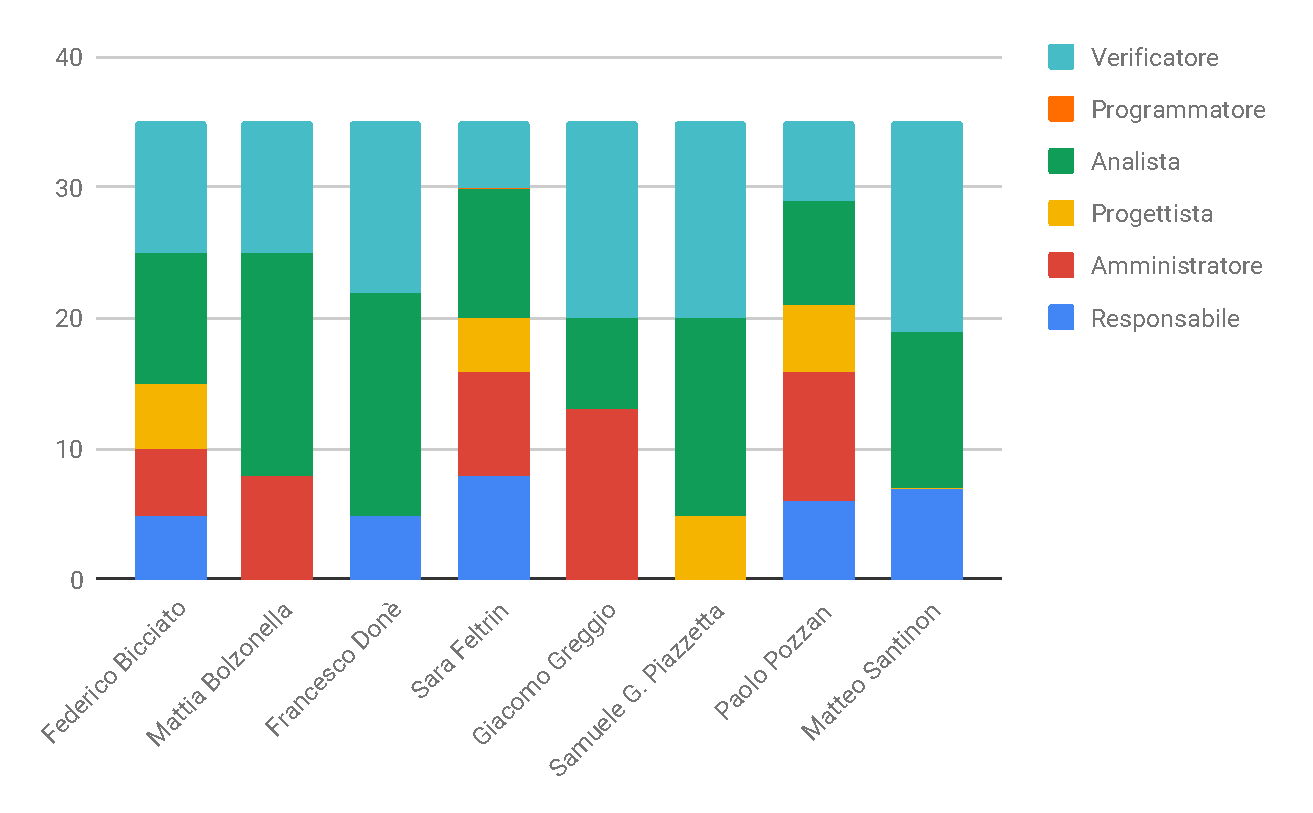
\includegraphics[width=0.9\textwidth]{res/images/istogramma_analisi.pdf}\\
				\caption{Istogramma della ripartizione di ore per ruolo in Analisi}
			\label{IstogrammaAnalisi}
\end{figure}


\subsubsection{Prospetto economico}
In questa fase il costo per ogni ruolo è il seguente:
\begin{table}[H]
	\centering\renewcommand{\arraystretch}{1.5}
	\caption{Prospetto dei costi per ruoli nel periodo di Analisi}
	\vspace{0.2cm}
    \begin{tabular}{c c c}
                   
    \rowcolorhead
     {\colorhead \textbf{Ruolo}} &
     {\colorhead \textbf{Ore}} & 
     {\colorhead \textbf{Costo}} \\
	
    \rowcolorlight
     {\colorbody Responsabile} & {\colorbody 31} & 
     {\colorbody \EUR{930,00}}  
	\\
	
	\rowcolordark
     {\colorbody Amministratore} & {\colorbody 44} & 
     {\colorbody \EUR{880,00}}
	\\	
	
	\rowcolorlight
     {\colorbody Analista} & {\colorbody 96} & 
     {\colorbody \EUR{2.400,00}} 
	\\
	
	\rowcolordark
     {\colorbody Progettista} & {\colorbody 19} & 
     {\colorbody \EUR{418,00}} 
	\\
	
	\rowcolorlight
     {\colorbody Programmatore} & {\colorbody -} & 
     {\colorbody -} 
	\\
	
	\rowcolordark
     {\colorbody Verificatore} & {\colorbody 90} & 
     {\colorbody \EUR{1.350,00}} 
	\\
	
	\rowcolorlight
     {\colorbody \textbf{Totale}} & {\colorbody 280} & 
     {\colorbody \EUR{5.978,00}} 
	
    \end{tabular} 
\end{table}
\pagebreak
I dati ottenuti si possono riassumere nel seguente areogramma:
\begin{figure}[H] 
\centering 
%	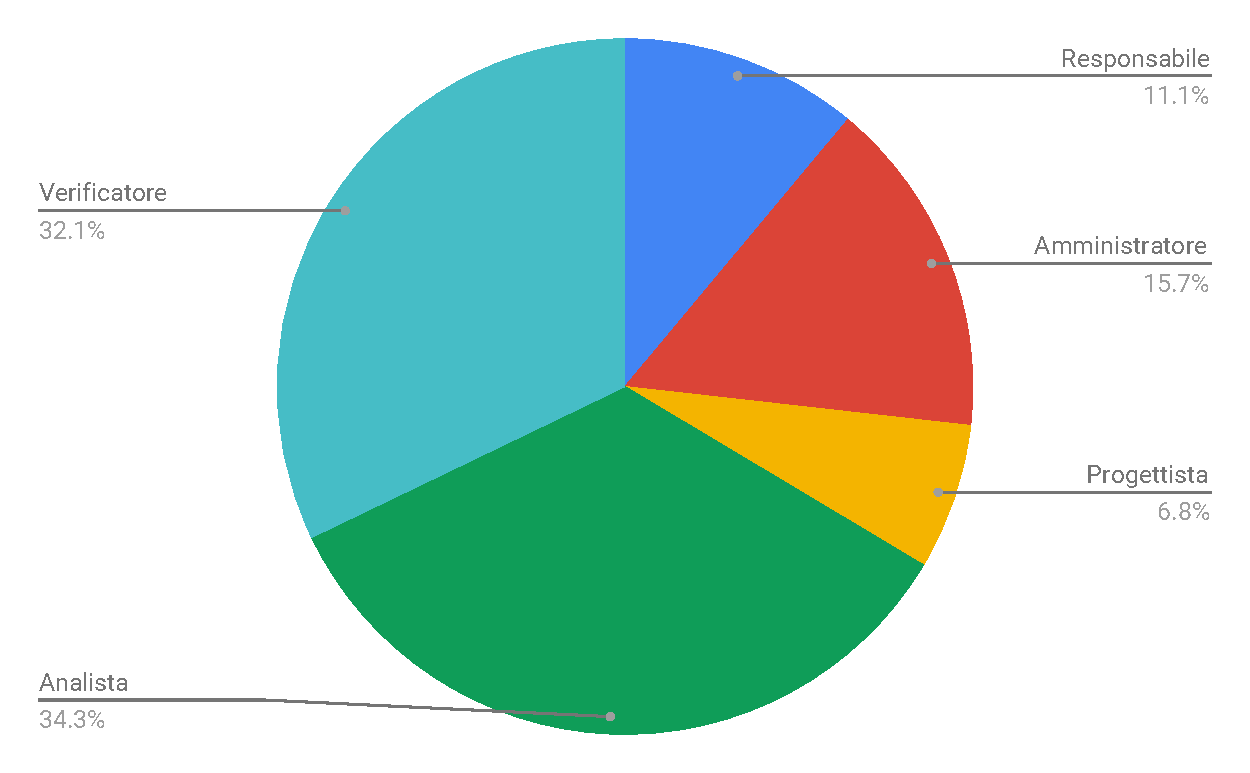
\includegraphics[width=0.7\textwidth]{res/images/areogramma_analisi.pdf}\\
	\caption{Areogramma della ripartizione di ore per ruolo in Analisi}
\label{AreogrammaAnalisi}
\end{figure}

\subsection{Fase di Consolidamento dei requisiti}
\subsubsection{Prospetto orario}
Il periodo di Consolidamento dei requisiti vede la seguente distribuzione oraria:
\begin{table}[H]
	\centering\renewcommand{\arraystretch}{1.5}
	\caption{Distribuzione delle ore nel periodo di Consolidamento 
		dei requisiti}
	\vspace{0.2cm}
    \begin{tabular}{c c c c c c c c}
                   
    \rowcolorhead
     {\colorhead \textbf{Nominativo}} &
     {\colorhead \textbf{Re}} & 
     {\colorhead \textbf{Am}} & 
     {\colorhead\textbf{An}} & 
     {\colorhead \textbf{Pt}} & 
     {\colorhead\textbf{Pr}} & 
     {\colorhead \textbf{Ve}} & 
     {\colorhead \textbf{Ore totali} }\\
	
    \rowcolorlight
     {\colorbody Federico Bicciato} & {\colorbody -} & 
     {\colorbody -} & {\colorbody 5} & {\colorbody -} & 
     {\colorbody -} & {\colorbody -} & {\colorbody 5} 
	\\
	
	\rowcolordark
     {\colorbody Mattia Bolzonella} & {\colorbody -} & 
     {\colorbody 5} & {\colorbody -} & {\colorbody -} & 
     {\colorbody -} & {\colorbody -} & {\colorbody 5} 
	\\	
	
	\rowcolorlight
     {\colorbody Francesco Donè} & {\colorbody -} & 
     {\colorbody -} & {\colorbody 2} & {\colorbody -} & 
     {\colorbody -} & {\colorbody 3} & {\colorbody 5} 
	\\
	
	\rowcolordark
     {\colorbody Sara Feltrin} & {\colorbody -} & 
     {\colorbody -} & {\colorbody 5} & {\colorbody -} & 
     {\colorbody -} & {\colorbody -} & {\colorbody 5} 
	\\
    
    \rowcolorlight
     {\colorbody Giacomo Greggio} & {\colorbody -} & 
     {\colorbody -} & {\colorbody -} & {\colorbody -} & 
     {\colorbody -} & {\colorbody 5} & {\colorbody 5} 
	\\
	
	\rowcolordark
     {\colorbody Samuele Giuliano Piazzetta} & {\colorbody 3} & 
     {\colorbody -} & {\colorbody -} & {\colorbody -} & 
     {\colorbody -} & {\colorbody 2} & {\colorbody 5} 
	\\	
	
	\rowcolorlight
     {\colorbody Paolo Pozzan} & {\colorbody -} & 
     {\colorbody -} & {\colorbody 3} & {\colorbody -} & 
     {\colorbody -} & {\colorbody 2} & {\colorbody 5} 
	\\
	
	\rowcolordark
     {\colorbody Matteo Santinon} & {\colorbody -} & 
     {\colorbody -} & {\colorbody -} & {\colorbody -} & 
     {\colorbody -} & {\colorbody 5} & {\colorbody 5} 
	\\
	
	\rowcolorlight
     {\colorbody \textbf{Ore totali ruolo}} & {\colorbody 3} & 
     {\colorbody 5} & {\colorbody 15} & {\colorbody -} & 
     {\colorbody -} & {\colorbody 17} & { \colorbody 40} 
	\\

    \end{tabular}           
\end{table}
\pagebreak
I dati ottenuti si possono riassumere nel seguente istogramma:
\begin{figure}[H] 
			\centering 
	%			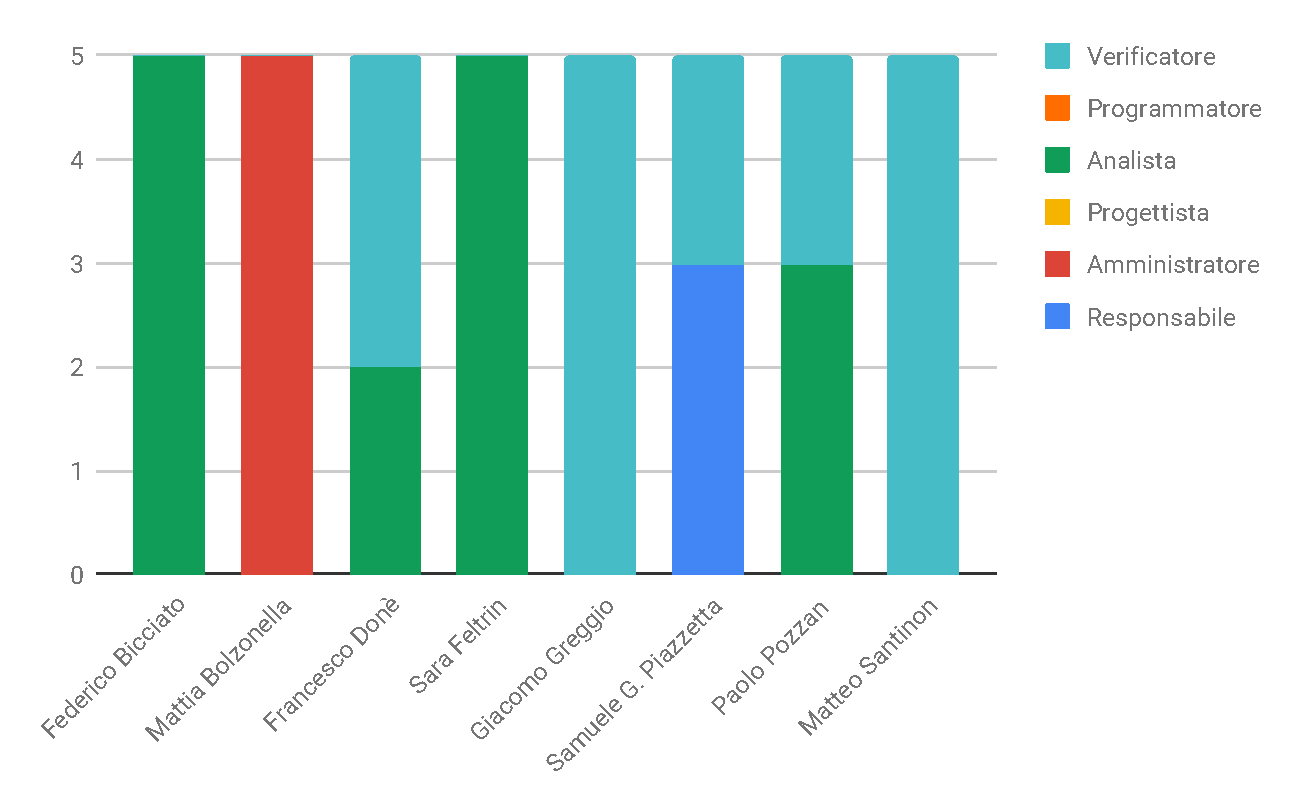
\includegraphics[width=0.9\textwidth]{res/images/istogramma_consolidamento.pdf}\\
				\caption{Istogramma della ripartizione di ore per ruolo in Consolidamento dei requisiti}
			\label{IstogrammaConsolidamento}
\end{figure}

\subsubsection{Prospetto economico}
In questa fase il costo per ogni ruolo è il seguente:
\begin{table}[H]
				\centering\renewcommand{\arraystretch}{1.5}
				\caption{Prospetto dei costi per ruoli nel periodo di 
					Consolidamento dei requisiti}
				\vspace{0.2cm}
                \begin{tabular}{c c c}
                               
                \rowcolorhead
                 {\colorhead \textbf{Ruolo}} &
                 {\colorhead \textbf{Ore}} & 
                 {\colorhead \textbf{Costo}} \\
				
                \rowcolorlight
                 {\colorbody Responsabile} & {\colorbody 3} & 
                 {\colorbody \EUR{90,00}}  
				\\
				
				\rowcolordark
                 {\colorbody Amministratore} & {\colorbody 5} & 
                 {\colorbody \EUR{100,00}}
				\\	
				
				\rowcolorlight
                 {\colorbody Analista} & {\colorbody 15} & 
                 {\colorbody \EUR{375,00}} 
				\\
				
				\rowcolordark
                 {\colorbody Progettista} & {\colorbody -} & 
                 {\colorbody -} 
				\\
				
				\rowcolorlight
                 {\colorbody Programmatore} & {\colorbody -} & 
                 {\colorbody -} 
				\\
				
				\rowcolordark
                 {\colorbody Verificatore} & {\colorbody 17} & 
                 {\colorbody \EUR{255,00}} 
				\\
				
				\rowcolorlight
                 {\colorbody \textbf{Totale}} & {\colorbody 40} & 
                 {\colorbody \EUR{820,00}} 
				\\
                

                \end{tabular}
                

\end{table}
\pagebreak
I dati ottenuti si possono riassumere nel seguente areogramma:
\begin{figure}[H] 
			\centering 
%				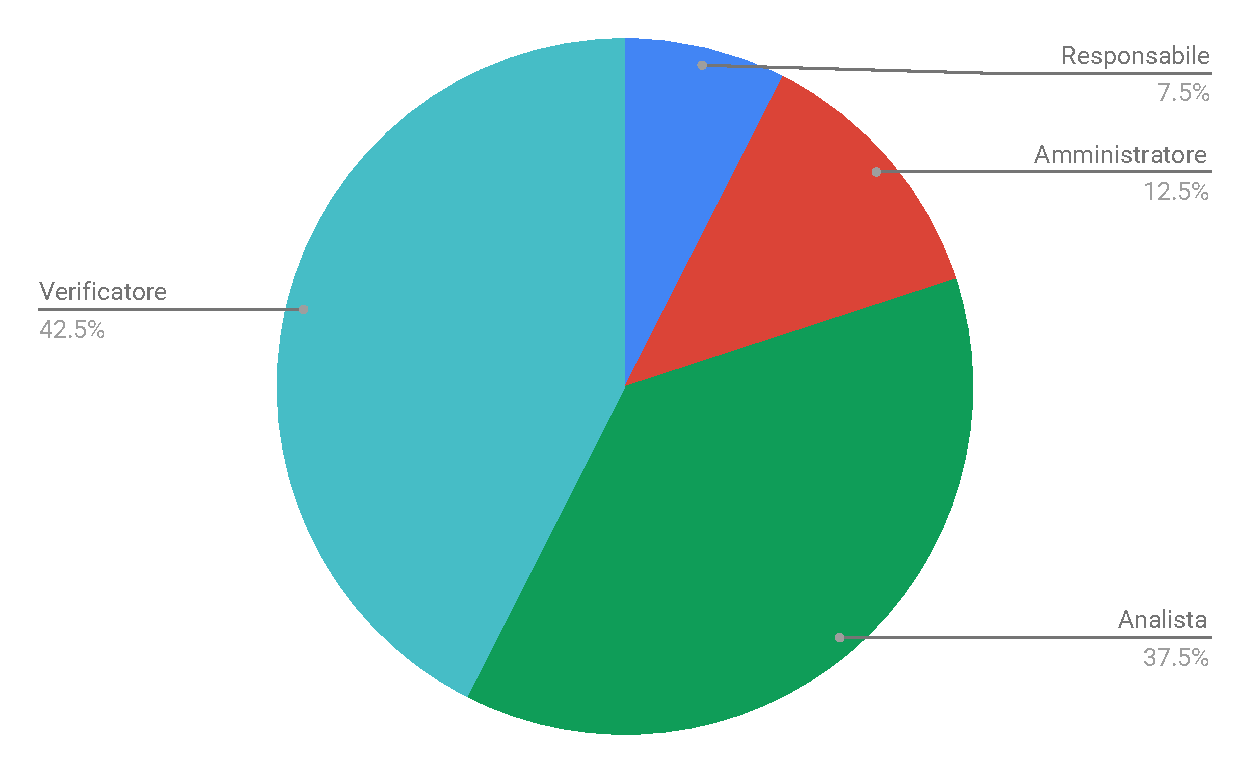
\includegraphics[width=0.7\textwidth]{res/images/areogramma_consolidamento.pdf}\\
				\caption{Areogramma della ripartizione di ore per ruolo in Consolidamento dei requisiti}
			\label{AreogrammaConsolidaemnto}
\end{figure}

\subsection{Fase di Progettazione architetturale}
\subsubsection{Prospetto orario}
Nella fase di Progettazione architetturale la distribuzione oraria è la seguente:
\begin{table}[H]
				\centering\renewcommand{\arraystretch}{1.5}
				\caption{Distribuzione delle ore nel periodo di Progettazione architetturale} 
				\vspace{0.2cm}
                \begin{tabular}{c c c c c c c c}
                              
                \rowcolorhead
                 {\colorhead \textbf{Nominativo}} &
                 {\colorhead \textbf{Re}} & 
                 {\colorhead \textbf{Am}} & 
                 {\colorhead\textbf{An}} & 
                 {\colorhead \textbf{Pt}} & 
                 {\colorhead\textbf{Pr}} & 
                 {\colorhead \textbf{Ve}} & 
                 {\colorhead \textbf{Ore totali} }\\
				
                \rowcolorlight
                 {\colorbody Federico Bicciato} & {\colorbody 6} & 
                 {\colorbody -} & {\colorbody 10} & {\colorbody -} & 
                 {\colorbody 6} & {\colorbody 6} & {\colorbody 28} 
				\\
				
				\rowcolordark
                 {\colorbody Mattia Bolzonella} & {\colorbody -} & 
                 {\colorbody -} & {\colorbody -} & {\colorbody 8} & 
                 {\colorbody 5} & {\colorbody 15} & {\colorbody 28} 
				\\	
			
				\rowcolorlight
                 {\colorbody Francesco Donè} & {\colorbody -} & 
                 {\colorbody 5} & {\colorbody -} & {\colorbody 7} & 
                 {\colorbody 6} & {\colorbody 10} & {\colorbody 28} 
				\\
					
				\rowcolordark
                 {\colorbody Sara Feltrin} & {\colorbody -} & 
                 {\colorbody 10} & {\colorbody -} & {\colorbody 5} & 
                 {\colorbody 5} & {\colorbody 8} & {\colorbody 28} 
				\\
                
                \rowcolorlight
                 {\colorbody Giacomo Greggio} & {\colorbody -} & 
                 {\colorbody 7} & {\colorbody -} & {\colorbody 15} & 
                 {\colorbody -} & {\colorbody 6} & {\colorbody 28} 
				\\
				
				\rowcolordark
                 {\colorbody Samuele Giuliano Piazzetta} & {\colorbody 4} & 
                 {\colorbody -} & {\colorbody 9} & {\colorbody 11} & 
                 {\colorbody 4} & {\colorbody -} & {\colorbody 28} 
				\\	
				
				\rowcolorlight
                 {\colorbody Paolo Pozzan} & {\colorbody -} & 
                 {\colorbody -} & {\colorbody 6} & {\colorbody 8} & 
                 {\colorbody 4} & {\colorbody 10} & {\colorbody 28} 
				\\
				
				\rowcolordark
                 {\colorbody Matteo Santinon} & {\colorbody -} & 
                 {\colorbody -} & {\colorbody 5} & {\colorbody 13} & 
                 {\colorbody -} & {\colorbody 10} & {\colorbody 28} 
				\\
				
				\rowcolorlight
                 {\colorbody \textbf{Ore totali ruolo}} & {\colorbody 10} & 
                 {\colorbody 22} & {\colorbody 30} & {\colorbody 67} & 
                 {\colorbody 30} & {\colorbody 65} & {\colorbody 224} 
				\\

                \end{tabular}             
\end{table}
\pagebreak
Una rappresentazione visiva della suddivisione oraria viene data dal seguente grafico:
\begin{figure}[H] 
			\centering 
		%		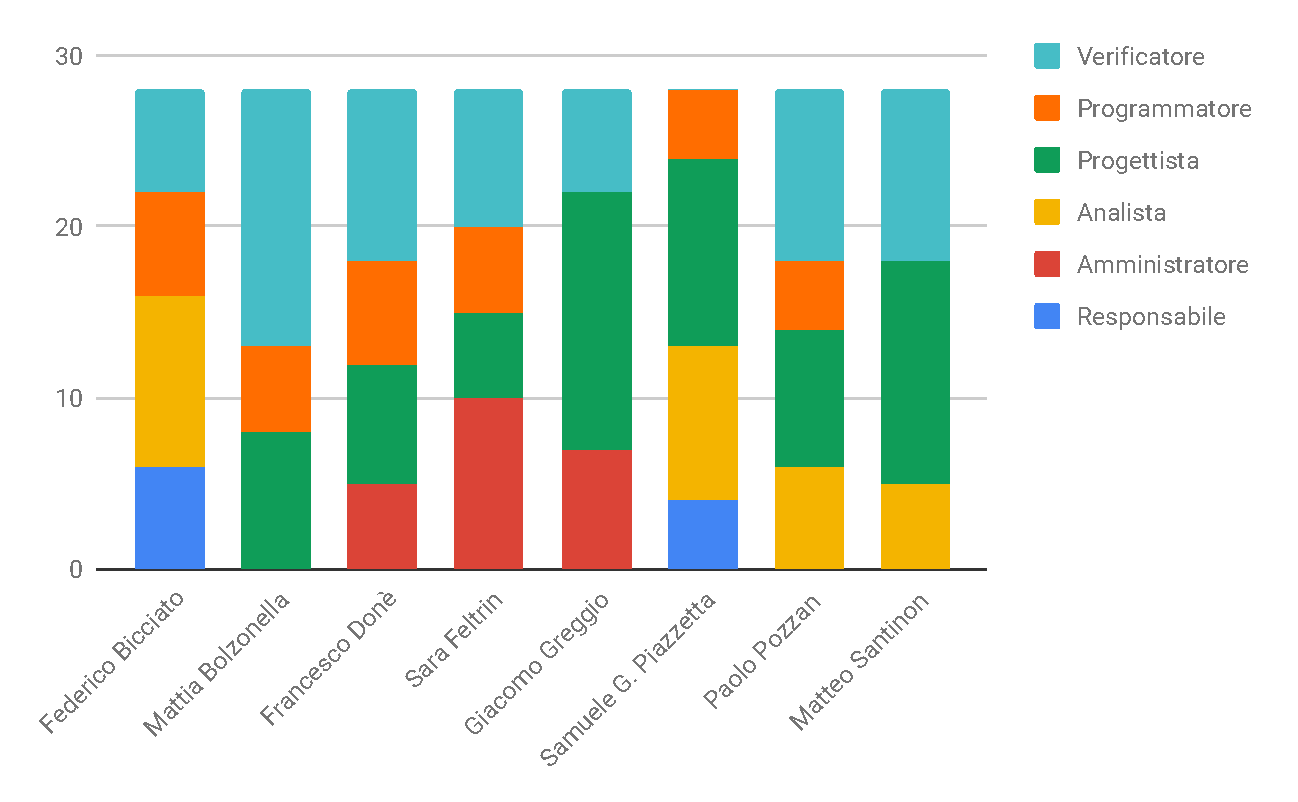
\includegraphics[width=0.9\textwidth]{res/images/istogramma_architetturale.pdf}\\
				\caption{Istogramma della ripartizione di ore per ruolo in Progettazione architetturale}
			\label{IstogrammaArchitetturale}
\end{figure}

\subsubsection{Prospetto economico}
In questa fase il costo per ogni ruolo è il seguente:
\begin{table}[H]
				\centering\renewcommand{\arraystretch}{1.5}
				\caption{Prospetto dei costi per ruoli nel periodo di 
					Progettazione architetturale}
				\vspace{0.2cm}
                \begin{tabular}{c c c}
                               
                \rowcolorhead
                 {\colorhead \textbf{Ruolo}} &
                 {\colorhead \textbf{Ore}} & 
                 {\colorhead \textbf{Costo}} \\
				
                \rowcolorlight
                 {\colorbody Responsabile} & {\colorbody 10} & 
                 {\colorbody \EUR{300,00}}  
				\\
				
				\rowcolordark
                 {\colorbody Amministratore} & {\colorbody 22} & 
                 {\colorbody \EUR{440,00}}
				\\	
				
				\rowcolorlight
                 {\colorbody Analista} & {\colorbody 30} & 
                 {\colorbody \EUR{750,00}} 
				\\
				
				\rowcolordark
                 {\colorbody Progettista} & {\colorbody 67} & 
                 {\colorbody \EUR{1.474,00}} 
				\\
				
				\rowcolorlight
                 {\colorbody Programmatore} & {\colorbody 30} & 
                 {\colorbody \EUR{450,00}} 
				\\
				
				\rowcolordark
                 {\colorbody Verificatore} & {\colorbody 65} & 
                 {\colorbody \EUR{975,00}} 
				\\
				
				\rowcolorlight
                 {\colorbody \textbf{Totale}} & {\colorbody 224} & 
                 {\colorbody \EUR{4.389,00}} 
				\\
                

                \end{tabular}
                

\end{table}
\pagebreak
I dati ottenuti si possono riassumere nel seguente areogramma:
\begin{figure}[H] 
			\centering 
%				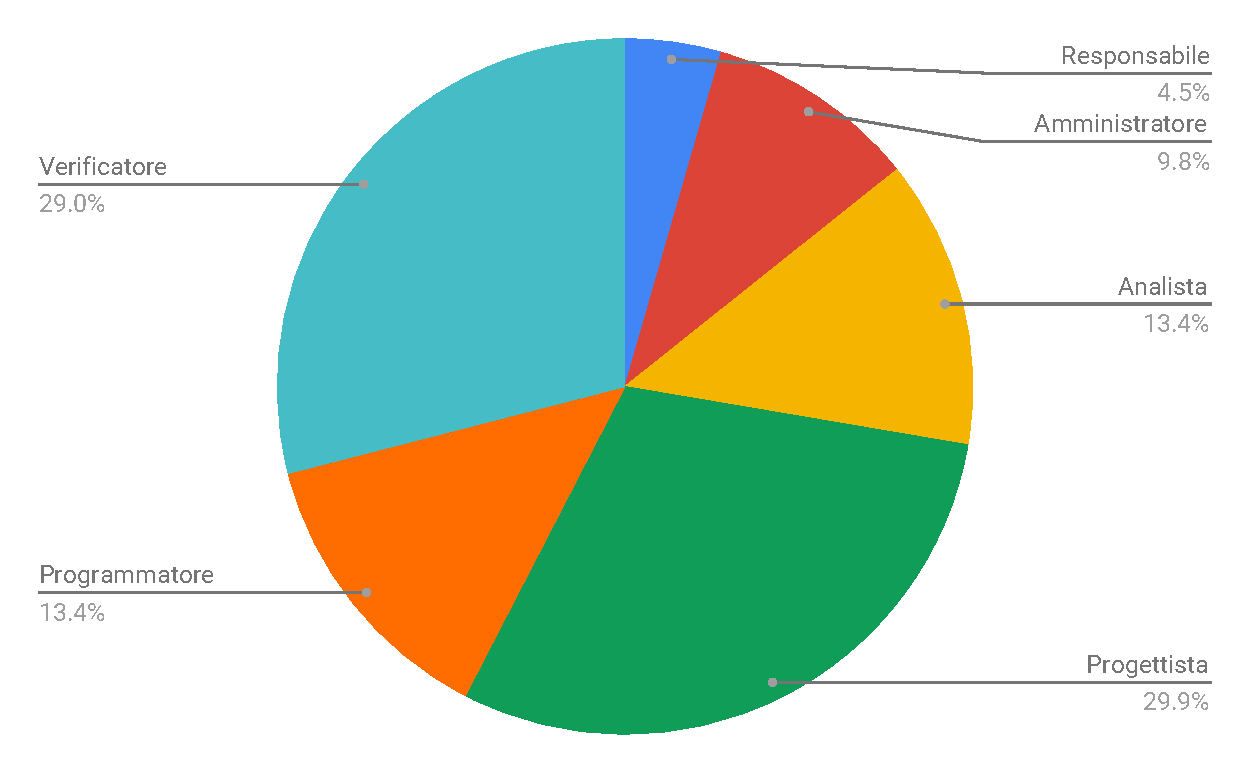
\includegraphics[width=0.7\textwidth]{res/images/areogramma_architetturale.pdf}\\
				\caption{Areogramma della ripartizione di ore per ruolo in Progettazione architetturale}
			\label{AreogrammaArchitetturale}
\end{figure}

\subsection{Fase di Progettazione di dettaglio e codifica}
\subsubsection{Prospetto orario}
Nella fase di Progettazione di dettaglio e codifica la distribuzione oraria è la seguente:
\begin{table}[H]
				\centering\renewcommand{\arraystretch}{1.5}
				\caption{Distribuzione delle ore nel periodo di Progettazione di dettaglio e codifica}
				\vspace{0.2cm}
                \begin{tabular}{c c c c c c c c}
                               
                \rowcolorhead
                 {\colorhead \textbf{Nominativo}} &
                 {\colorhead \textbf{Re}} & 
                 {\colorhead \textbf{Am}} & 
                 {\colorhead\textbf{An}} & 
                 {\colorhead \textbf{Pt}} & 
                 {\colorhead\textbf{Pr}} & 
                 {\colorhead \textbf{Ve}} & 
                 {\colorhead \textbf{Ore totali} }\\
				
                \rowcolorlight
                 {\colorbody Federico Bicciato} & {\colorbody -} & 
                 {\colorbody 8} & {\colorbody -} & {\colorbody 8} & 
                 {\colorbody 20} & {\colorbody 14} & {\colorbody 50} 
				\\
				
				\rowcolordark
                 {\colorbody Mattia Bolzonella} & {\colorbody 8} & 
                 {\colorbody 3} & {\colorbody -} & {\colorbody 6} & 
                 {\colorbody 20} & {\colorbody 13} & {\colorbody 50} 
				\\	
				
				\rowcolorlight
                 {\colorbody Francesco Donè} & {\colorbody 4} & 
                 {\colorbody 4} & {\colorbody -} & {\colorbody 12} & 
                 {\colorbody 20} & {\colorbody 10} & {\colorbody 50} 
				\\
				
				\rowcolordark
                 {\colorbody Sara Feltrin} & {\colorbody -} & 
                 {\colorbody -} & {\colorbody -} & {\colorbody 15} & 
                 {\colorbody 21} & {\colorbody 14} & { \colorbody 50} 
				\\
                
                \rowcolorlight
                 {\colorbody Giacomo Greggio} & {\colorbody 4} & 
                 {\colorbody 6} & {\colorbody -} & {\colorbody 8} & 
                 {\colorbody 16} & {\colorbody 16} & {\colorbody 50} 
				\\
				
				\rowcolordark
                 {\colorbody Samuele Giuliano Piazzetta} & {\colorbody -} & 
                 {\colorbody -} & {\colorbody -} & {\colorbody 15} & 
                 {\colorbody 20} & {\colorbody 15} & {\colorbody 50} 
				\\	
				
				\rowcolorlight
                 {\colorbody Paolo Pozzan} & {\colorbody 5} & 
                 {\colorbody -} & {\colorbody -} & {\colorbody 15} & 
                 {\colorbody 20} & {\colorbody 10} & {\colorbody 50} 
				\\
				
				\rowcolordark
                 {\colorbody Matteo Santinon} & {\colorbody -} & 
                 {\colorbody 8} & {\colorbody -} & {\colorbody 11} & 
                 {\colorbody 20} & {\colorbody 11} & {\colorbody 50} 
				\\
				
				\rowcolorlight
                 {\colorbody \textbf{Ore totali ruolo}} & {\colorbody 21} & 
                 {\colorbody 29} & {\colorbody -} & {\colorbody 90} & 
                 {\colorbody 157} & {\colorbody 103} & {\colorbody 400} 
				\\

                \end{tabular}
                

\end{table}
\pagebreak
Una rappresentazione visiva della suddivisione oraria viene data dal seguente grafico:
\begin{figure}[H] 
			\centering 
		%		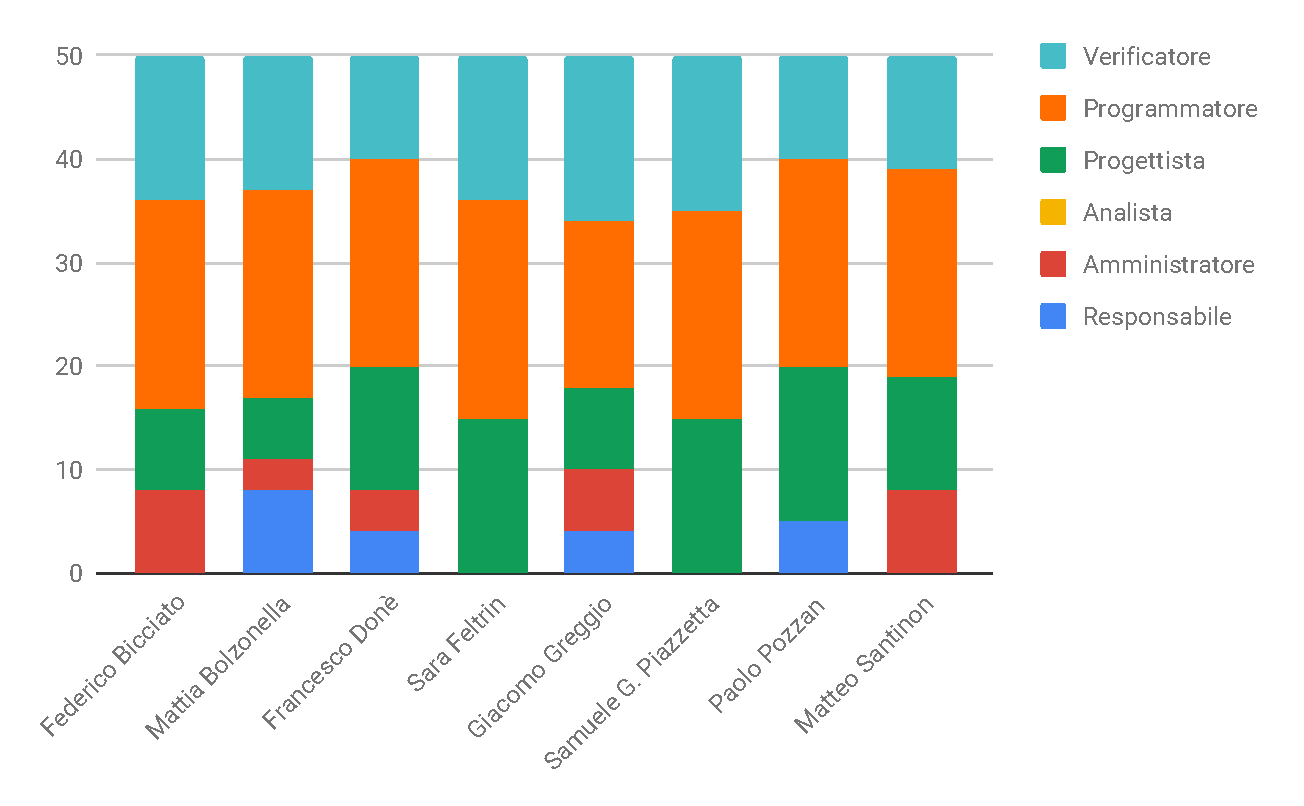
\includegraphics[width=0.9\textwidth]{res/images/istogramma_dettaglio.pdf}\\
				\caption{Istogramma della ripartizione di ore per ruolo in Progettazione di dettaglio e codifica}
			\label{IstogrammaDettaglio}
\end{figure}

\subsubsection{Prospetto economico}
In questa fase il costo per ogni ruolo è il seguente:
\begin{table}[H]
				\centering\renewcommand{\arraystretch}{1.5}
				\caption{Prospetto dei costi per ruoli nel periodo di 
					Progettazione di dettaglio e codifica}
				\vspace{0.2cm}
                \begin{tabular}{c c c}
                               
                \rowcolorhead
                 {\colorhead \textbf{Ruolo}} &
                 {\colorhead \textbf{Ore}} & 
                 {\colorhead \textbf{Costo}} \\
				
                \rowcolorlight
                 {\colorbody Responsabile} & {\colorbody 21} & 
                 {\colorbody \EUR{630,00}}  
				\\
				
				\rowcolordark
                 {\colorbody Amministratore} & {\colorbody 29} & 
                 {\colorbody \EUR{580,00}}
				\\	
				
				\rowcolorlight
                 {\colorbody Analista} & {\colorbody -} & 
                 {\colorbody -} 
				\\
				
				\rowcolordark
                 {\colorbody Progettista} & {\colorbody 90} & 
                 {\colorbody \EUR{1.980,00}} 
				\\
				
				\rowcolorlight
                 {\colorbody Programmatore} & {\colorbody 157} & 
                 {\colorbody \EUR{2.355,00}} 
				\\
				
				\rowcolordark
                 {\colorbody Verificatore} & {\colorbody 103} & 
                 {\colorbody \EUR{1.545,00}} 
				\\
				
				\rowcolorlight
                 {\colorbody \textbf{Totale}} & {\colorbody 400} & 
                 {\colorbody \EUR{7.090,00}} 
				\\
                

                \end{tabular}
                

\end{table}
\pagebreak
I dati ottenuti si possono riassumere nel seguente areogramma:
\begin{figure}[H] 
			\centering 
			%	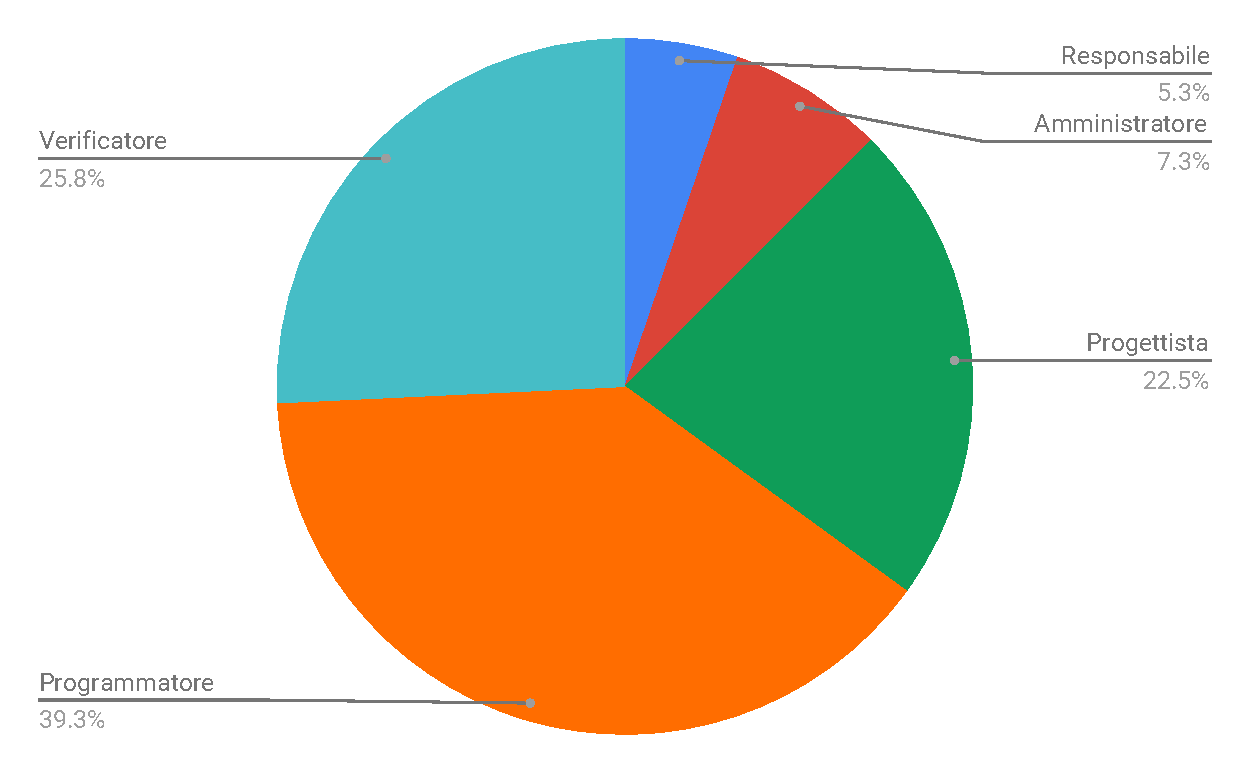
\includegraphics[width=0.7\textwidth]{res/images/areogramma_dettaglio.pdf}\\
				\caption{Areogramma della ripartizione di ore per ruolo in Progettazione di dettaglio e codifica}
			\label{AreogrammaDettaglio}
\end{figure}


\subsection{Fase di Validazione e collaudo}
\subsubsection{Prospetto orario}
Nella fase di progettazione di Validazione e collaudo la distribuzione oraria è la seguente:
\begin{table}[H]
				\centering\renewcommand{\arraystretch}{1.5}
				\caption{Distribuzione delle ore nel periodo di Validazione e 
					collaudo}
				\vspace{0.2cm}
                \begin{tabular}{c c c c c c c c}
                               
                \rowcolorhead
                 {\colorhead \textbf{Nominativo}} &
                 {\colorhead \textbf{Re}} & 
                 {\colorhead \textbf{Am}} & 
                 {\colorhead\textbf{An}} & 
                 {\colorhead \textbf{Pt}} & 
                 {\colorhead\textbf{Pr}} & 
                 {\colorhead \textbf{Ve}} & 
                 {\colorhead \textbf{Ore totali} }\\
				
                \rowcolorlight
                 {\colorbody Federico Bicciato} & {\colorbody -} & 
                 {\colorbody -} & {\colorbody -} & {\colorbody 5} & 
                 {\colorbody 5} & {\colorbody 10} & {\colorbody 20} 
				\\
				
				\rowcolordark
                 {\colorbody Mattia Bolzonella} & {\colorbody -} & 
                 {\colorbody -} & {\colorbody -} & {\colorbody 4} & 
                 {\colorbody 6} & {\colorbody 10} & {\colorbody 20} 
				\\	
				
				\rowcolorlight
                 {\colorbody Francesco Donè} & {\colorbody 4} & 
                 {\colorbody 5} & {\colorbody -} & {\colorbody -} & 
                 {\colorbody 5} & {\colorbody 6} & {\colorbody 20} 
				\\
				
				\rowcolordark
                 {\colorbody Sara Feltrin} & {\colorbody 4} & 
                 {\colorbody -} & {\colorbody -} & {\colorbody -} & 
                 {\colorbody 4} & {\colorbody 12} & {\colorbody 20} 
				\\
                
                \rowcolorlight
                 {\colorbody Giacomo Greggio} & {\colorbody 5} & 
                 {\colorbody -} & {\colorbody -} & {\colorbody -} & 
                 {\colorbody 7} & {\colorbody 8} & {\colorbody 20} 
				\\
				
				\rowcolordark
                 {\colorbody Samuele Giuliano Piazzetta} & {\colorbody -} & 
                 {\colorbody 6} & {\colorbody -} & {\colorbody -} & 
                 {\colorbody 8} & {\colorbody 6} & {\colorbody 20} 
				\\	
				
				\rowcolorlight
                 {\colorbody Paolo Pozzan} & {\colorbody -} & 
                 {\colorbody 5} & {\colorbody -} & {\colorbody 5} & 
                 {\colorbody -} & {\colorbody 10} & {\colorbody 20} 
				\\
				
				\rowcolordark
                 {\colorbody Matteo Santinon} & {\colorbody 4} & 
                 {\colorbody -} & {\colorbody -} & {\colorbody -} & 
                 {\colorbody 6} & {\colorbody 10} & {\colorbody 20} 
				\\
				
				\rowcolorlight
                 {\colorbody \textbf{Ore totali ruolo}} & {\colorbody 17} & 
                 {\colorbody 16} & {\colorbody -} & {\colorbody 14} & 
                 {\colorbody 41} & {\colorbody 72} & {\colorbody 160} 
				\\

                \end{tabular}
                
\end{table}
\pagebreak
Una rappresentazione visiva della suddivisione oraria viene data dal seguente grafico:
\begin{figure}[H] 
			\centering 
		%		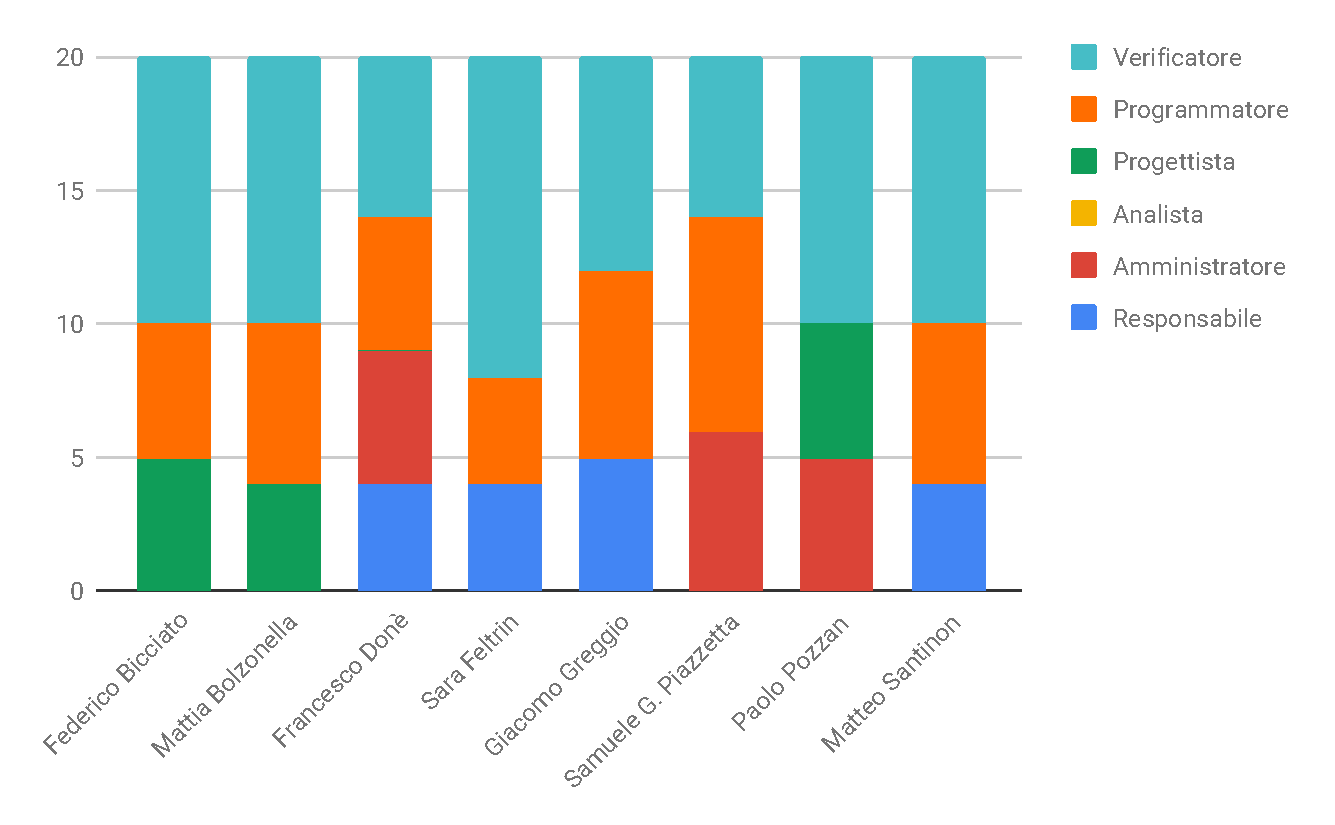
\includegraphics[width=0.9\textwidth]{res/images/istogramma_validazione.pdf}\\
				\caption{Istogramma della ripartizione di ore per ruolo in Validazione e collaudo}
			\label{IstogrammaValidazione}
\end{figure}

\subsubsection{Prospetto economico}
In questa fase il costo per ogni ruolo è il seguente:
\begin{table}[H]
				\centering\renewcommand{\arraystretch}{1.5}
				\caption{Prospetto dei costi per ruoli nel periodo di 
					Validazione e collaudo}
				\vspace{0.2cm}
                \begin{tabular}{c c c}
                               
                \rowcolorhead
                 {\colorhead \textbf{Ruolo}} &
                 {\colorhead \textbf{Ore}} & 
                 {\colorhead \textbf{Costo}} \\
				
                \rowcolorlight
                 {\colorbody Responsabile} & {\colorbody 17} & 
                 {\colorbody \EUR{510,00}}  
				\\
				
				\rowcolordark
                 {\colorbody Amministratore} & {\colorbody 16} & 
                 {\colorbody \EUR{320,00}}
				\\	
				
				\rowcolorlight
                 {\colorbody Analista} & {\colorbody -} & 
                 {\colorbody -} 
				\\
				
				\rowcolordark
                 {\colorbody Progettista} & {\colorbody 14} & 
                 {\colorbody \EUR{308,00}} 
				\\
				
				\rowcolorlight
                 {\colorbody Programmatore} & {\colorbody 41} & 
                 {\colorbody \EUR{615,00}} 
				\\
				
				\rowcolordark
                 {\colorbody Verificatore} & {\colorbody 72} & 
                 {\colorbody \EUR{1.080,00}} 
				\\
				
				\rowcolorlight
                 {\colorbody \textbf{Totale}} & {\colorbody 160} & 
                 {\colorbody \EUR{2.833,00}} 
				\\
                

                \end{tabular}
                

\end{table}
\pagebreak
I dati ottenuti si possono riassumere nel seguente areogramma:
\begin{figure}[H] 
			\centering 
		%		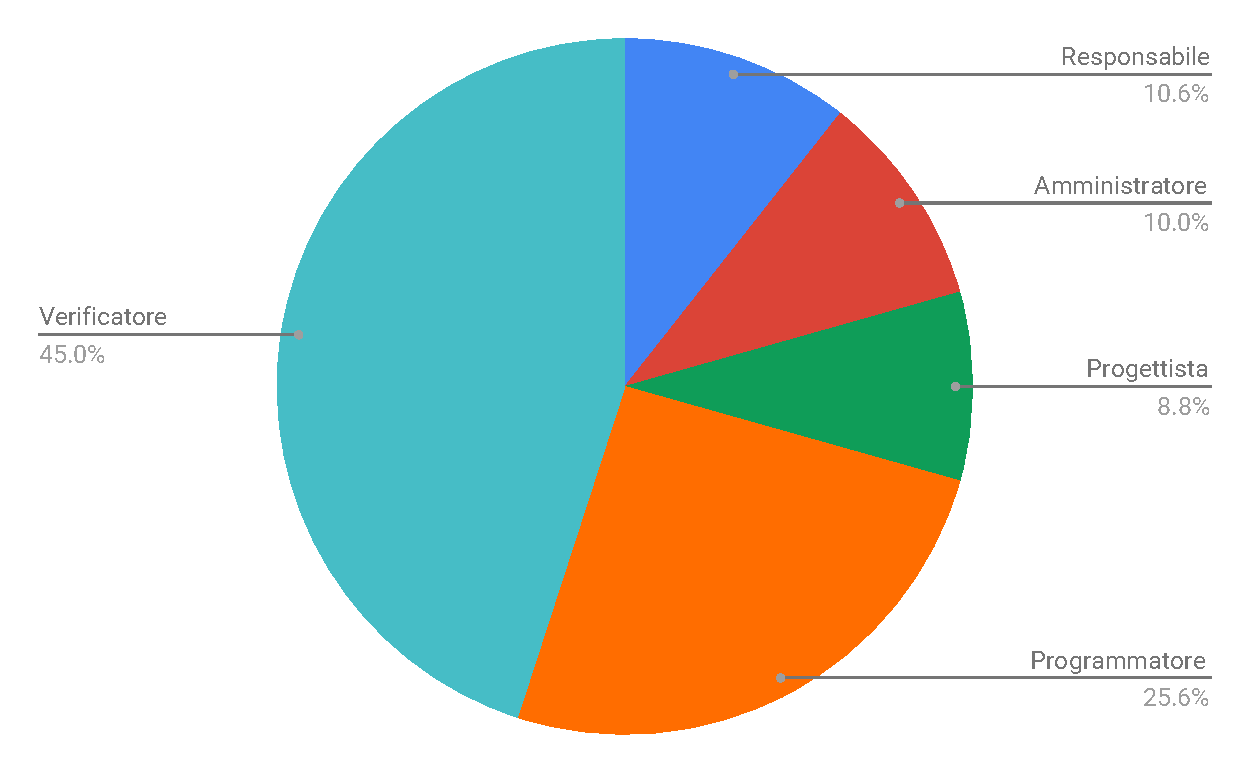
\includegraphics[width=0.7\textwidth]{res/images/areogramma_validazione.pdf}\\
				\caption{Areogramma della ripartizione di ore per ruolo in Validazione e collaudo}
			\label{AreogrammaValidazione}
\end{figure}


\subsection{Riepilogo}
\subsubsection{Ore totali}
\paragraph{Suddivisione del lavoro}\mbox{}\\
Vengono riportate il totale delle ore del progetto in cui sono presenti le ore di investimento e le ore rendicontate a carico del committente:
\begin{table}[H]
				\centering\renewcommand{\arraystretch}{1.5}
				\caption{Distribuzione delle ore totali di investimento e rendicontate}
				\vspace{0.2cm}
                \begin{tabular}{c c c c c c c c}
                               
                \rowcolorhead
                 {\colorhead \textbf{Nominativo}} &
                 {\colorhead \textbf{Re}} & 
                 {\colorhead \textbf{Am}} & 
                 {\colorhead\textbf{An}} & 
                 {\colorhead \textbf{Pt}} & 
                 {\colorhead\textbf{Pr}} & 
                 {\colorhead \textbf{Ve}} & 
                 {\colorhead \textbf{Ore totali} }\\
				
                \rowcolorlight
                 {\colorbody Federico Bicciato} & {\colorbody 11} & 
                 {\colorbody 13} & {\colorbody 25} & {\colorbody 18} & 
                 {\colorbody 31} & {\colorbody 40} & {\colorbody 138} 
				\\
				
				\rowcolordark
                 {\colorbody Mattia Bolzonella} & {\colorbody 8} & 
                 {\colorbody 16} & {\colorbody 17} & {\colorbody 18} & 
                 {\colorbody 31} & {\colorbody 48} & {\colorbody 138} 
				\\	
				
				\rowcolorlight
                 {\colorbody Francesco Donè} & {\colorbody 13} & 
                 {\colorbody 14} & {\colorbody 19} & {\colorbody 19} & 
                 {\colorbody 31} & {\colorbody 42} & {\colorbody 138} 
				\\
				
				\rowcolordark
                 {\colorbody Sara Feltrin} & {\colorbody 12} & 
                 {\colorbody 18} & {\colorbody 15} & {\colorbody 24} & 
                 {\colorbody 30} & {\colorbody 39} & {\colorbody 138} 
				\\
                
                \rowcolorlight
                 {\colorbody Giacomo Greggio} & {\colorbody 9} & 
                 {\colorbody 26} & {\colorbody 7} & {\colorbody 23} & 
                 {\colorbody 23} & {\colorbody 50} & {\colorbody 138} 
				\\
				
				\rowcolordark
                 {\colorbody Samuele Giuliano Piazzetta} & {\colorbody 7} & 
                 {\colorbody 6} & {\colorbody 24} & {\colorbody 31} & 
                 {\colorbody 32} & {\colorbody 38} & {\colorbody 138} 
				\\	
				
				\rowcolorlight
                 {\colorbody Paolo Pozzan} & {\colorbody 11} & 
                 {\colorbody 15} & {\colorbody 17} & {\colorbody 33} & 
                 {\colorbody 24} & {\colorbody 38} & {\colorbody 138} 
				\\
				
				\rowcolordark
                 {\colorbody Matteo Santinon} & {\colorbody 11} & 
                 {\colorbody 8} & {\colorbody 17} & {\colorbody 24} & 
                 {\colorbody 26} & {\colorbody 52} & {\colorbody 138} 
				\\
				
				\rowcolorlight
                 {\colorbody \textbf{Ore totali ruolo}} & {\colorbody 82} & 
                 {\colorbody 116} & {\colorbody 141} & {\colorbody 190} & 
                 {\colorbody 228} & {\colorbody 347} & {\colorbody 1104} 
				\\

                \end{tabular}
                

\end{table}
\pagebreak
Una rappresentazione visiva della suddivisione oraria viene data dal seguente grafico:
\begin{figure}[H] 
			\centering 
			%	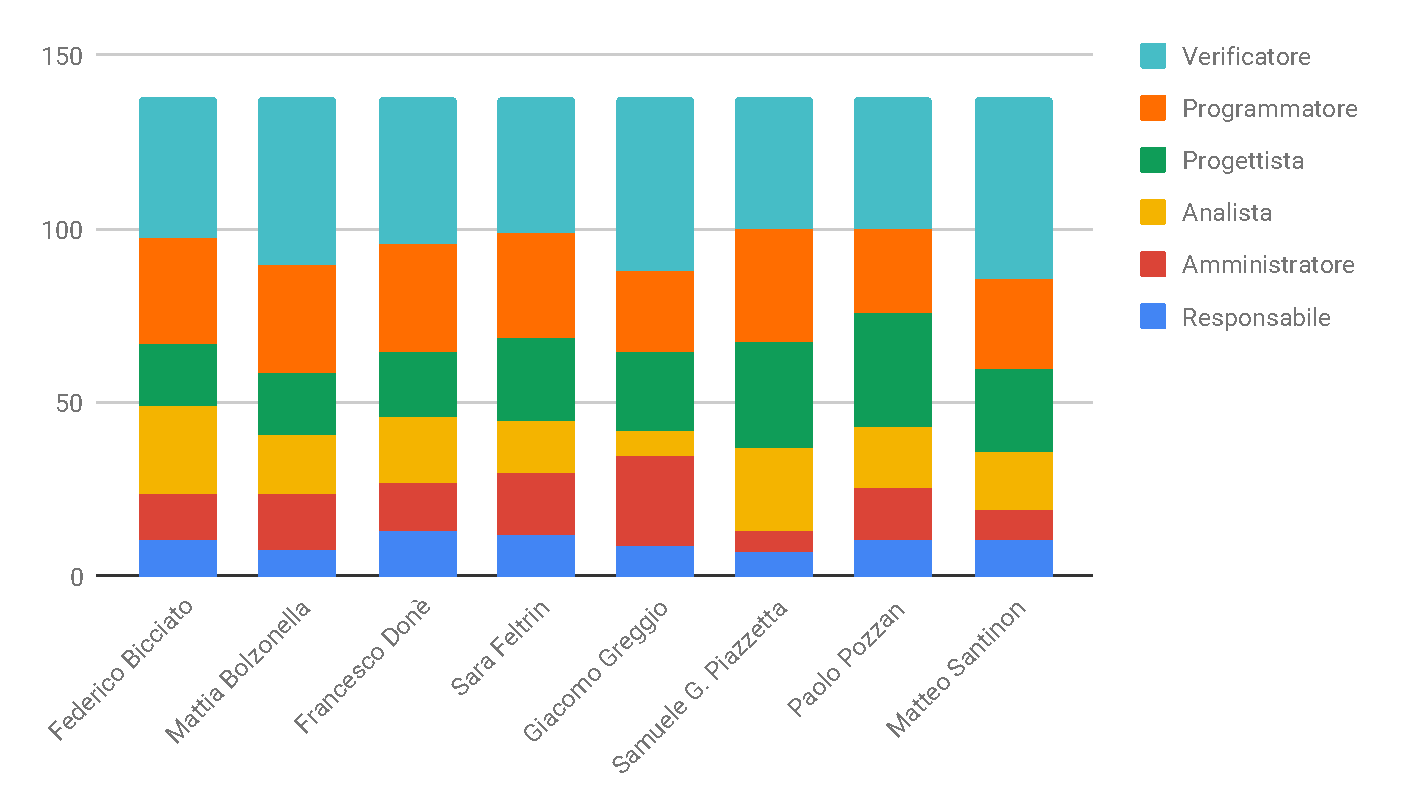
\includegraphics[width=0.9\textwidth]{res/images/istogramma_riepilogo.pdf}\\
				\caption{Istogramma della ripartizione di ore totali di investimento e rendicontate}
			\label{IstogrammaRiepilogo}
\end{figure}

\paragraph{Prospetto economico}\mbox{}\\
In questa fase il costo per ogni ruolo è il seguente:
\begin{table}[H]
				\centering\renewcommand{\arraystretch}{1.5}
				\caption{Prospetto dei costi totale delle ore di investimento e rendicontate}
				\vspace{0.2cm}
                \begin{tabular}{c c c}
                               
                \rowcolorhead
                 {\colorhead \textbf{Ruolo}} &
                 {\colorhead \textbf{Ore}} & 
                 {\colorhead \textbf{Costo}} \\
				
                \rowcolorlight
                 {\colorbody Responsabile} & {\colorbody 82} & 
                 {\colorbody \EUR{2.460,00}}  
				\\
				
				\rowcolordark
                 {\colorbody Amministratore} & {\colorbody 116} & 
                 {\colorbody \EUR{2.320,00}}
				\\	
				
				\rowcolorlight
                 {\colorbody Analista} & {\colorbody 141} & 
                 {\colorbody \EUR{3.525,00}} 
				\\
				
				\rowcolordark
                 {\colorbody Progettista} & {\colorbody 190} & 
                 {\colorbody \EUR{4.180,00}} 
				\\
				
				\rowcolorlight
                 {\colorbody Programmatore} & {\colorbody 228} & 
                 {\colorbody \EUR{3.420,00}} 
				\\
				
				\rowcolordark
                 {\colorbody Verificatore} & {\colorbody 347} & 
                 {\colorbody \EUR{5.205,00}} 
				\\
				
				\rowcolorlight
                 {\colorbody \textbf{Totale}} & {\colorbody 1104} & 
                 {\colorbody \EUR{21.110,00}} 
				\\
                

                \end{tabular}
                

\end{table}
\pagebreak
I dati ottenuti si possono riassumere nel seguente areogramma:
\begin{figure}[H] 
			\centering 
		%		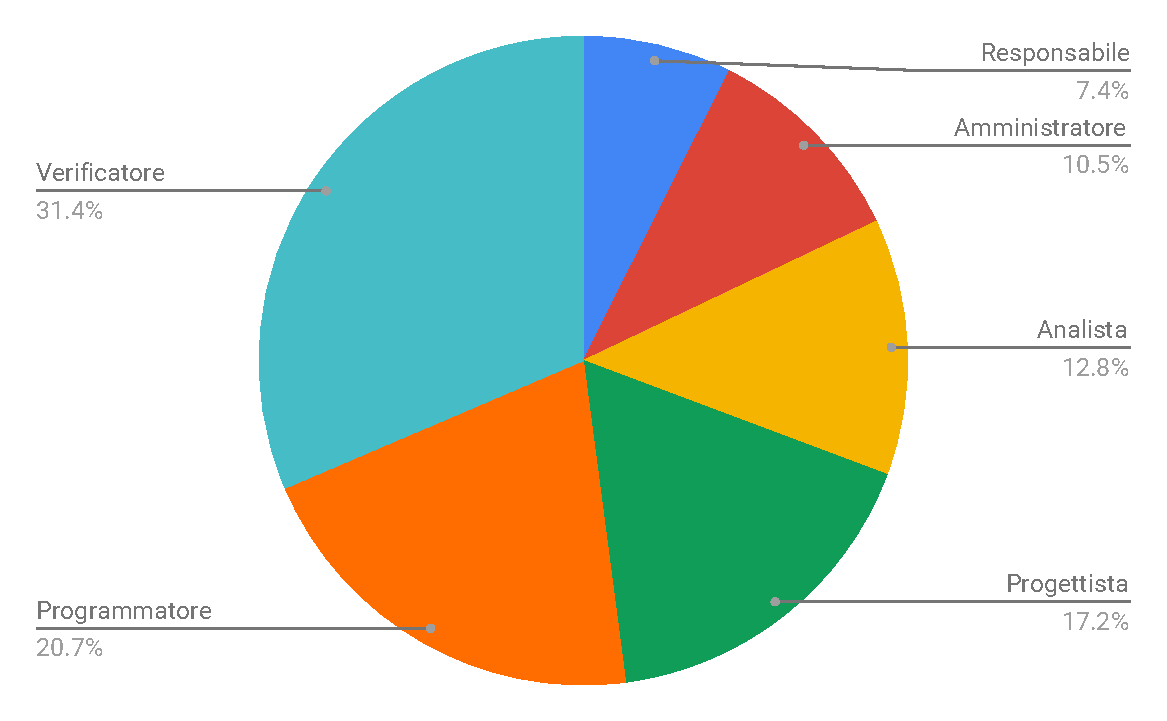
\includegraphics[width=0.7\textwidth]{res/images/areogramma_riepilogo.pdf}\\
				\caption{Areogramma dei costi totale delle ore di investimento e rendicontate}
			\label{AreogrammaRiepilogoRuoli}
\end{figure}


\subsubsection{Ore rendicontate}
\paragraph{Suddivisione del lavoro}\mbox{}\\
\linebreak
Le ore rendicontate sono riassunte nella seguente tabella:
\begin{table}[H]
				\centering\renewcommand{\arraystretch}{1.5}
				\caption{Distribuzione delle ore rendicontate}
				\vspace{0.2cm}
                \begin{tabular}{c c c c c c c c}
                               
                \rowcolorhead
                 {\colorhead \textbf{Nominativo}} &
                 {\colorhead \textbf{Re}} & 
                 {\colorhead \textbf{Am}} & 
                 {\colorhead\textbf{An}} & 
                 {\colorhead \textbf{Pt}} & 
                 {\colorhead\textbf{Pr}} & 
                 {\colorhead \textbf{Ve}} & 
                 {\colorhead \textbf{Ore totali} }\\
				
                \rowcolorlight
                 {\colorbody Federico Bicciato} & {\colorbody 6} & 
                 {\colorbody 8} & {\colorbody 15} & {\colorbody 13} & 
                 {\colorbody 31} & {\colorbody 30} & {\colorbody 103} 
				\\
				
				\rowcolordark
                 {\colorbody Mattia Bolzonella} & {\colorbody 8} & 
                 {\colorbody 8} & {\colorbody -} & {\colorbody 18} & 
                 {\colorbody 31} & {\colorbody 38} & {\colorbody 103} 
				\\	
				
				\rowcolorlight
                 {\colorbody Francesco Donè} & {\colorbody 8} & 
                 {\colorbody 14} & {\colorbody 2} & {\colorbody 19} & 
                 {\colorbody 31} & {\colorbody 29} & {\colorbody 103} 
				\\
				
				\rowcolordark
                 {\colorbody Sara Feltrin} & {\colorbody 4} & 
                 {\colorbody 10} & {\colorbody 5} & {\colorbody 20} & 
                 {\colorbody 30} & {\colorbody 34} & {\colorbody 103} 
				\\
                
                \rowcolorlight
                 {\colorbody Giacomo Greggio} & {\colorbody 9} & 
                 {\colorbody 13} & {\colorbody -} & {\colorbody 23} & 
                 {\colorbody 23} & {\colorbody 35} & {\colorbody 103} 
				\\
				
				\rowcolordark
                 {\colorbody Samuele Giuliano Piazzetta} & {\colorbody 7} & 
                 {\colorbody 6} & {\colorbody 9} & {\colorbody 26} & 
                 {\colorbody 32} & {\colorbody 23} & {\colorbody 103} 
				\\	
				
				\rowcolorlight
                 {\colorbody Paolo Pozzan} & {\colorbody 5} & 
                 {\colorbody 5} & {\colorbody 9} & {\colorbody 28} & 
                 {\colorbody 24} & {\colorbody 32} & {\colorbody 103} 
				\\
				
				\rowcolordark
                 {\colorbody Matteo Santinon} & {\colorbody 4} & 
                 {\colorbody 8} & {\colorbody 5} & {\colorbody 24} & 
                 {\colorbody 26} & {\colorbody 36} & {\colorbody 103} 
				\\
				
				\rowcolorlight
                 {\colorbody \textbf{Ore totali ruolo}} & {\colorbody 51} & 
                 {\colorbody 72} & {\colorbody 45} & {\colorbody 171} & 
                 {\colorbody 228} & {\colorbody 257} & {\colorbody 824} 
				\\

                \end{tabular}
                

\end{table}

\begin{figure}[H] 
			\centering 
			%	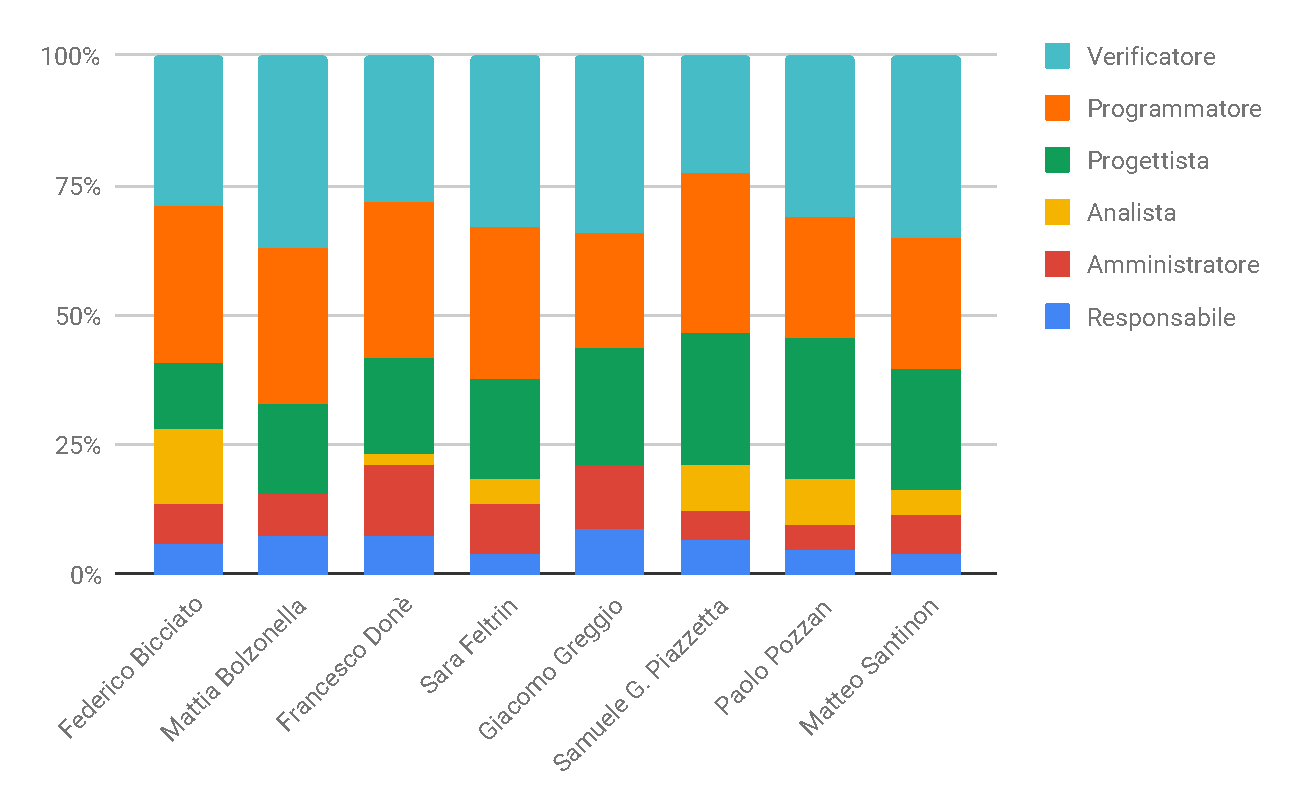
\includegraphics[width=0.9\textwidth]{res/images/istogramma_rendicontate.pdf}\\
				\caption{Istogramma della ripartizione delle ore rendicontate}
			\label{IstogrammaOreRendicontate}
\end{figure}

\paragraph{Prospetto economico}\mbox{}\\
\linebreak
Il totale rendicontato dei costi sostenuti per ogni ruolo è riassunto nella seguente tabella:

\begin{table}[H]
				\centering\renewcommand{\arraystretch}{1.5}
				\caption{Prospetto dei costi delle ore rendicontate}
				\vspace{0.2cm}
                \begin{tabular}{c c c}
                               
                \rowcolorhead
                 {\colorhead \textbf{Ruolo}} &
                 {\colorhead \textbf{Ore}} & 
                 {\colorhead \textbf{Costo}} \\
				
                \rowcolorlight
                 {\colorbody Responsabile} & {\colorbody 51} & 
                 {\colorbody \EUR{1.530,00}}  
				\\
				
				\rowcolordark
                 {\colorbody Amministratore} & {\colorbody 72} & 
                 {\colorbody \EUR{1.440,00}}
				\\	
				
				\rowcolorlight
                 {\colorbody Analista} & {\colorbody 45} & 
                 {\colorbody \EUR{1.125,00}} 
				\\
				
				\rowcolordark
                 {\colorbody Progettista} & {\colorbody 171} & 
                 {\colorbody \EUR{3.762,00}} 
				\\
				
				\rowcolorlight
                 {\colorbody Programmatore} & {\colorbody 228} & 
                 {\colorbody \EUR{3.420,00}} 
				\\
				
				\rowcolordark
                 {\colorbody Verificatore} & {\colorbody 257} & 
                 {\colorbody \EUR{3.855,00}} 
				\\
				
				\rowcolorlight
                 {\colorbody \textbf{Totale}} & {\colorbody 824} & 
                 {\colorbody \EUR{15.132,00}} 
				\\
                

                \end{tabular}
                

\end{table}
\pagebreak
I dati ottenuti si possono riassumere nel seguente areogramma:
\begin{figure}[H] 
			\centering 
		%		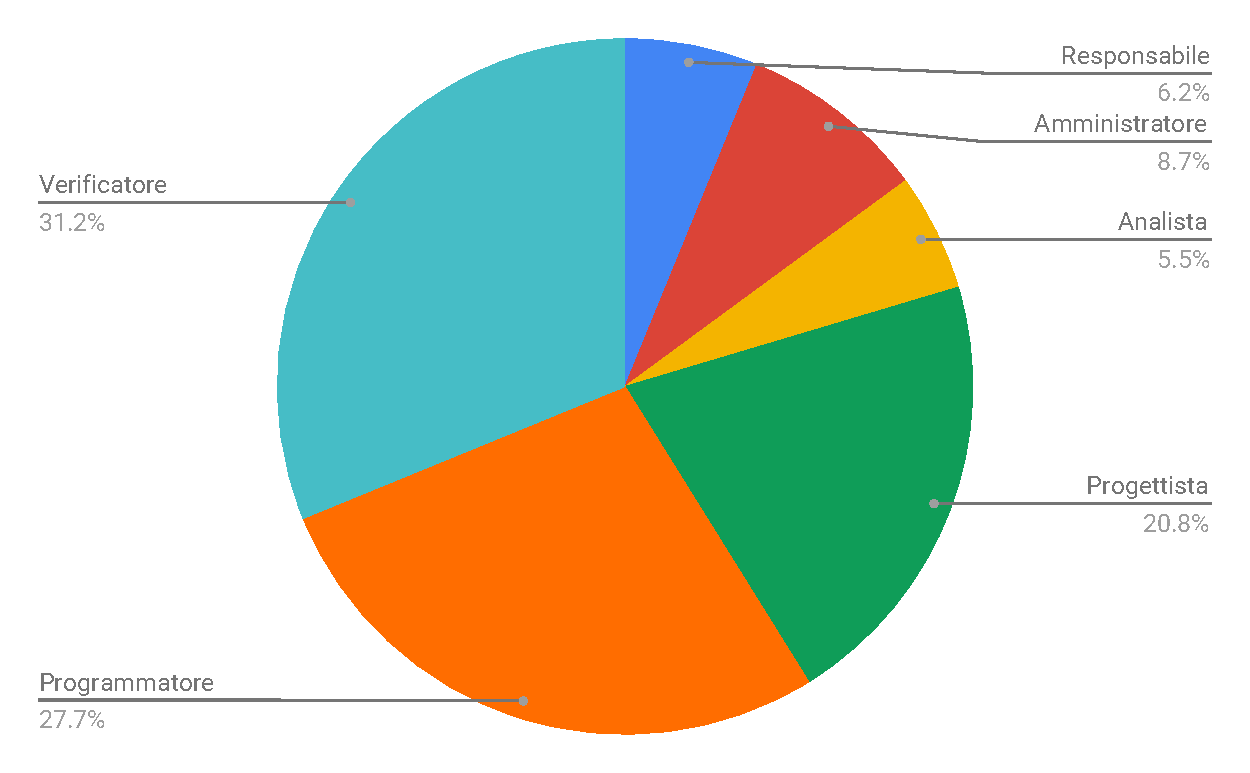
\includegraphics[width=0.7\textwidth]{res/images/areogramma_rendicontate.pdf}\\
				\caption{Areogramma delle ore rendicontate per ruolo}
			\label{AreogrammaOreRendicontate}
\end{figure}

\subsubsection{Conclusioni}
Il costo totale preventivato per il progetto è \EUR{15.132,00}.



\pagebreak
\section{Consuntivi di periodo}
Di seguito verranno indicate le spese effettivamente sostenute, considerando sia quelle per ruolo sia quelle per persona. Il bilancio potrà risultare:
\begin{itemize}
	\item \textbf{Positivo:} se il preventivo supera il consuntivo;
	\item \textbf{Pari:} se il consuntivo e il preventivo sono pari;
	\item \textbf{Negativo:} se il consuntivo supera il preventivo.
\end{itemize}

\subsection{Periodo di analisi}
Le ore di lavoro sostenute in questa fase sono da considerarsi come ore di investimento per l'approfondimento personale. Esse sono quindi non rendicontate.

\begin{table}[H]
				\centering\renewcommand{\arraystretch}{1.5}
				\caption{Consuntivo di periodo della fase di analisi}
				\vspace{0.2cm}
                \begin{tabular}{c c c}
                               
                \rowcolorhead
                 {\colorhead \textbf{Ruolo}} &
                 {\colorhead \textbf{Ore}} & 
                 {\colorhead \textbf{Costo}} \\
				
                \rowcolorlight
                 {\colorbody Responsabile} & {\colorbody 38 (+2)} & 
                 {\colorbody \EUR{1.140,00} (+\EUR{60,00})}  
				\\
				
				\rowcolordark
                 {\colorbody Amministratore} & {\colorbody 25 (+7)} & 
                 {\colorbody \EUR{500,00} (+\EUR{140,00})}
				\\	
				
				\rowcolorlight
                 {\colorbody Analista} & {\colorbody 71 (-4)} & 
                 {\colorbody \EUR{1.775,00} (-\EUR{100,00})} 
				\\
				
				\rowcolordark
                 {\colorbody Progettista} & {\colorbody 19
                 (+0)} & 
                 {\colorbody \EUR{418,00} (+\EUR{0,00})} 
				\\
				
				\rowcolorlight
                 {\colorbody Programmatore} & {\colorbody -} & 
                 {\colorbody -} 
				\\
				
				\rowcolordark
                 {\colorbody Verificatore} & {\colorbody 57 (+3)} & 
                 {\colorbody \EUR{855,00} (+\EUR{45,00})} 
				\\
				
				\rowcolorlight
                 {\colorbody \textbf{Totale Preventivo}} & {\colorbody \textbf{210}} & 
                 {\colorbody \textbf{\EUR{4.688,00}}} 
				\\
				
				
				\rowcolordark
                 {\colorbody \textbf{Totale Consuntivo}} & {\colorbody \textbf{218}} & 
                 {\colorbody \textbf{\EUR{4.833,00}}} 
				\\
				
				
				\rowcolorlight
                 {\colorbody \textbf{Differenza}} & {\colorbody \textbf{8}} & 
                 {\colorbody \textbf{\EUR{+145,00}}} 
				\\
				
                

                \end{tabular}
                
\end{table}

\subsubsection{Conclusioni}
Come emerge dai dati riportati nella tabella soprastante, che presenta le ore relative al consuntivo della fase di Analisi, è stato necessario investire più tempo del previsto nei ruoli di \textit{Responsabile}, \textit{Amministratore} e \textit{Verificatore}.  Al contempo però sono risultate sufficienti
un numero inferiore di ore per il ruolo di \textit{Analista}. 
Di seguito sono elencate le cause dei ritardi sopracitati:
\begin{itemize}
	\item \textbf{Amministratori:} la ricerca e configurazione dei software atti alla produzione e alla gestione del progetto ha richiesto più tempo del previsto, in particolare la creazione dei template \LaTeX\space e la configurazione di PragmaDb\glo;\
	\item \textbf{Responsabile:} si è reso necessario un monte ore maggiore per la coordinazione generale del progetto, causato dall'inesperienza dei membri del gruppo; 
	\item \textbf{Verificatore:} a causa dell'inesperienza dei membri del gruppo si sono verificati diversi errori e mancanze durante la stesura della documentazione che hanno richiesto un maggiore monte ore di verifica;
	\item \textbf{Analista:} al contrario di quanto preventivato il totale delle ore di analisi è risultato inferiore, questo grazie alla facile comprensione dei requisiti richiesti che ha permesso una rapida stesura di quest'ultimi.
\end{itemize}

\subsubsection{Preventivo a finire}
Il risultato del periodo è complessivamente di 8 ore lavorative oltre il previsto e di una
spesa aggiunta di \EUR{+145,00}, che però facendo parte del periodo di investimento
non influirà sul totale rendicontato.

\subsection{Periodo di consolidamento dei requisiti}
Le ore di lavoro sostenute durante questo periodo sono successive alla fase di analisi. Diverse ore sono state impiegate per lo studio personale delle tecnologie che andremo ad utilizzare e per questo non vengono riportate nella tabella sottostante e non sono rendicontate.


\begin{table}[H]
	\centering\renewcommand{\arraystretch}{1.5}
	\caption{Consuntivo di periodo della fase di consolidamento dei requisiti}
	\vspace{0.2cm}
	\begin{tabular}{c c c}
		
		\rowcolorhead
		{\colorhead \textbf{Ruolo}} &
		{\colorhead \textbf{Ore}} & 
		{\colorhead \textbf{Costo}} \\
		
		\rowcolorlight
		{\colorbody Responsabile} & {\colorbody 5 (+0)} & 
		{\colorbody \EUR{150,00} (+\EUR{0,00})}  
		\\
		
		\rowcolordark
		{\colorbody Amministratore} & {\colorbody 3 (+0)} & 
		{\colorbody \EUR{60,00} (+\EUR{0,00})}
		\\	
		
		\rowcolorlight
		{\colorbody Analista} & {\colorbody 12 (+0)} & 
		{\colorbody \EUR{300,00} (+\EUR{0,00})} 
		\\
		
		\rowcolordark
		{\colorbody Progettista} & {\colorbody -} & 
		{\colorbody \EUR{0,00} (+\EUR{0,00})} 
		\\
		
		\rowcolorlight
		{\colorbody Programmatore} & {\colorbody -} & 
		{\colorbody -} 
		\\
		
		\rowcolordark
		{\colorbody Verificatore} & {\colorbody 10 (+0)} & 
		{\colorbody \EUR{150,00} (+\EUR{0,00})} 
		\\
		
		\rowcolorlight
		{\colorbody \textbf{Totale Preventivo}} & {\colorbody \textbf{30}} & 
		{\colorbody \textbf{\EUR{660,00}}} 
		\\
		
		
		\rowcolordark
		{\colorbody \textbf{Totale Consuntivo}} & {\colorbody \textbf{30}} & 
		{\colorbody \textbf{\EUR{660,00}}} 
		\\
		
		
		\rowcolorlight
		{\colorbody \textbf{Differenza}} & {\colorbody -} & 
		{\colorbody -} 
		\\
		
		
		
	\end{tabular}
	
\end{table}

\subsubsection{Conclusioni}
Come emerge dai dati riportati nella tabella soprastante, che presenta le ore relative al consuntivo della fase di Consolidamento dei requisiti, è stato rispettato il monte ore preventivato. Questo grazie all'esperienza acquisita durante la fase precedente e alla breve durata del periodo, che ha permesso una migliore gestione delle risorse.

\subsubsection{Preventivo a finire}
Il risultato del consuntivo di periodo coincide col monte ore preventivato inoltre, facendo parte del periodo rendicontato, non è necessario eseguire nessuna modifica o accorgimenti ai futuri periodo o al preventivo.

\subsection{Periodo di progettazione e codifica per la Technology Baseline}
Le ore di lavoro sostenute durante questo periodo sono successive alla fase di analisi. Diverse ore sono state impiegate per lo studio personale delle tecnologie che andremo ad utilizzare e per questo non vengono riportate nella tabella sottostante e non sono rendicontate.


\begin{table}[H]
	\centering\renewcommand{\arraystretch}{1.5}
	\caption{Consuntivo di periodo della fase di progettazione e codifica per la Technology Baseline}
	\vspace{0.2cm}
	\begin{tabular}{c c c}
		
		\rowcolorhead
		{\colorhead \textbf{Ruolo}} &
		{\colorhead \textbf{Ore}} & 
		{\colorhead \textbf{Costo}} \\
		
		\rowcolorlight
		{\colorbody Responsabile} & {\colorbody 10 (+0)} & 
		{\colorbody \EUR{300,00} (+\EUR{0,00})}  
		\\
		
		\rowcolordark
		{\colorbody Amministratore} & {\colorbody 17 (+10)} & 
		{\colorbody \EUR{540,00} (+\EUR{200,00})}
		\\	
		
		\rowcolorlight
		{\colorbody Analista} & {\colorbody 29 (-5)} & 
		{\colorbody \EUR{625,00} (-\EUR{100,00})} 
		\\
		
		\rowcolordark
		{\colorbody Progettista} & {\colorbody 41 (-20)} & 
		{\colorbody \EUR{462,00} (-\EUR{440,00})} 
		\\
		
		\rowcolorlight
		{\colorbody Programmatore} & {\colorbody 26 (+35)} & 
		{\colorbody \EUR{915,00} (+\EUR{525,00})} 
		\\
		
		\rowcolordark
		{\colorbody Verificatore} & {\colorbody 45 (-20)} & 
		{\colorbody \EUR{375,00} (-\EUR{300,00})} 
		\\
		
		\rowcolorlight
		{\colorbody \textbf{Totale Preventivo}} & {\colorbody \textbf{168}} & 
		{\colorbody \textbf{\EUR{3332,00}}} 
		\\
		
		
		\rowcolordark
		{\colorbody \textbf{Totale Consuntivo}} & {\colorbody \textbf{168}} & 
		{\colorbody \textbf{\EUR{3192,00}}} 
		\\
		
		
		\rowcolorlight
		{\colorbody \textbf{Differenza}} & {\colorbody -} & 
		{\colorbody \textbf{+\EUR{140,00}}} 
		\\
		
		
		
	\end{tabular}
	
\end{table}

\subsubsection{Conclusioni}
Come emerge dai dati riportati nella tabella soprastante, che presenta le ore relative al consuntivo della fase di Progettazione e Codifica per la Technology Baseline, la progettazione ha subito una sostanziale modifica. Tale scostamento è dovuto all'idea iniziale di presentare una completa progettazione architetturale del prodotto. Tuttavia ci siamo concentrati maggiormente sul creare delle solide fondamenta per lo sviluppo dell'applicazione attraverso la progettazione e codifica del Proof of Concept\glo. Di seguito sono riportate in dettaglio i vari scostamenti orari dei ruoli interessati:
\begin{itemize}
\item \textbf{Amministratori:} successivamente alla fase di testing dell'editor prestabilito sono insorte svariate problematiche riguardanti il sistema di Continuos Integration\glo, che ha richiesto un notevole monte ore per essere operativo;
\item \textbf{Progettista:} visto il cambiamento dell'obbiettivo finale di questo periodo il monte ore per la fase di progettazione è diminuito in quanto il progettista ha dovuto occuparsi solo di alcune parti del prodotto finale; 
\item \textbf{Verificatore:} a seguito della diminuzione del monte ore della fase di progettazione anche la fase di verifica ha subito una diminuzione del monte ore totali preventivate;
\item \textbf{Programmatore:} al contrario di quanto preventivato il totale delle ore di programmazione ha subito un notevole aumento, ciò è dovuto alla necessità di integrare le modifiche da noi apportate con il codice dell'applicazione già fornito dal proponente. La difficoltà di tale integrazione è scaturita dalla difficoltà di comprensione di alcune parti del codice fornito prive di documentazione e/o semplici commenti.
\end{itemize}

\subsubsection{Preventivo a finire}
Il bilancio economico è positivo, sono stati risparmiati \EUR{140,00}. Tali fondi verranno reinvestiti nelle fasi future per la realizzazione di alcuni requisiti opzionali.


\subsection{Periodo di progettazione di dettaglio e codifica}
Le ore sostenute durante questo periodo sono relative alla redazione alla codifica necessaria per la realizzazione della Product Baseline\glo. Tale periodo è da considerarsi rendicontato in quanto il lavoro è svolto con lo scopo di sviluppare il prodotto finale.


\begin{table}[H]
	\centering\renewcommand{\arraystretch}{1.5}
	\caption{Consuntivo di periodo della fase di progettazione di dettaglio e codifica}
	\vspace{0.2cm}
	\begin{tabular}{c c c}
		
		\rowcolorhead
		{\colorhead \textbf{Ruolo}} &
		{\colorhead \textbf{Ore}} & 
		{\colorhead \textbf{Costo}} \\
		
		\rowcolorlight
		{\colorbody Responsabile} & {\colorbody 16 (+0)} & 
		{\colorbody \EUR{480,00} (+\EUR{0,00})}  
		\\
		
		\rowcolordark
		{\colorbody Amministratore} & {\colorbody 21 (-5)} & 
		{\colorbody \EUR{420,00} (-\EUR{100,00})}
		\\	
		
		\rowcolorlight
		{\colorbody Analista} & {\colorbody 0 (+7)} & 
		{\colorbody \EUR{0,00} (+\EUR{125,00})} 
		\\
		
		\rowcolordark
		{\colorbody Progettista} & {\colorbody 64 (+20)} & 
		{\colorbody \EUR{1408,00} (+\EUR{440,00})} 
		\\
		
		\rowcolorlight
		{\colorbody Programmatore} & {\colorbody 117 (+10)} & 
		{\colorbody \EUR{1755,00} (+\EUR{150,00})} 
		\\
		
		\rowcolordark
		{\colorbody Verificatore} & {\colorbody 82 (+0)} & 
		{\colorbody \EUR{1230,00} (+\EUR{0,00})} 
		\\
		
		\rowcolorlight
		{\colorbody \textbf{Totale Preventivo}} & {\colorbody \textbf{300}} & 
		{\colorbody \textbf{\EUR{5293,00}}} 
		\\
		
		
		\rowcolordark
		{\colorbody \textbf{Totale Consuntivo}} & {\colorbody \textbf{332}} & 
		{\colorbody \textbf{\EUR{6258,00}}} 
		\\
		
		
		\rowcolorlight
		{\colorbody \textbf{Differenza}} & {\colorbody \textbf{32}} & 
		{\colorbody \textbf{+\EUR{965,00}}} 
		\\
		\rowcolordark
		{\colorbody \textbf{Totale con risparmio(-\EUR{140,00})}} & & 
		{\colorbody \textbf{\EUR{825,00}}} 
		\\
		
		
	\end{tabular}
	
\end{table}

\subsubsection{Conclusioni}
Come emerge dai dati riportati nella tabella soprastante, che presenta le ore relative al consuntivo della fase di Progettazione di Dettaglio e Codifica, la progettazione ha subito una sostanziale modifica. Di seguito sono riportati in dettaglio i vari scostamenti orari dei ruoli interessati:
\begin{itemize}
	\item \textbf{Amministratori:} sono stati risolti i probelmi sorti nella fase precedente riguardanti la Continuos Integration\glosp ciò ha portato ad una diminuzione del monte ore preventivato;
	\item \textbf{Progettista:} si è reso necessario un monte ore maggiore per questo ruolo a causa della necessità di individuare i corretti design pattern\glosp da applicare, soprattuto per quanto riguarda il back end\glo. Modifica che ci è stata suggerita a seguito della Product Baseline\glo; 
	\item \textbf{Verificatore:} nonostante la variazione del monte ore da programmatore le ore preventivate sono risultate sufficienti;
	\item \textbf{Programmatore:} al contrario di quanto preventivato il totale delle ore di programmazione ha subito un leggero aumento, a causa della difficoltà di integrare alcune parti riguardanti la Gamification\glo, e di alcune modifiche richieste dalla proponente.
\end{itemize}

Di seguito riportiamo la tabella riguardante l'avanzamento degli incrementi individuati in questa fase. Come si può notare lo sviluppo della maggior parte degli incrementi raggiunge la quasi totalità di completamento. Prendiamo come esempio la Gestione Veicoli, la quale è completa e funzionante ma necessita dell'integrazione della parte di Gamification\glosp per essere ultimata. Quest'ultima riguarderà un altro incremento che verrà sviluppato nella fase successiva.

\counterwithin{table}{section}
\renewcommand{\arraystretch}{1.5}
\rowcolors{2}{dispari}{pari}
\arrayrulecolor{white}
\begin{longtable}{ 
		>{\centering}p{0.17\textwidth} 
		>{\raggedright}p{0.28\textwidth}
		>{\raggedright}p{0.29\textwidth} 
		>{\centering}p{0.15\textwidth}
	}
	
	
	\caption{Tabella del completamento degli incrementi}\\
	\rowcolorhead
	\colorhead\textbf{Incremento} & \centering\colorhead\textbf{Completamento(\%)}
	\tabularnewline
	\endfirsthead
	\rowcolor{white}\caption[]{(continua)}\\
	\rowcolorhead
	\colorhead\textbf{Incremento} & \centering\colorhead\textbf{Completamento(\%)}
	\tabularnewline
	\endhead
	
	%R---------------------------------------------------------
	{Lucky Spin} & \centering 100\\
	\tabularnewline
	
	%R---------------------------------------------------------
	{Daily Rewards} & \centering 100\\
	\tabularnewline
	
	%R---------------------------------------------------------
	{Milestone Unlock} & \centering 100\\
	\tabularnewline
	%R---------------------------------------------------------
	{Leaderboard} & \centering 100\\
	\tabularnewline
	%R---------------------------------------------------------
	{Codice Invita Amici}\\ & \centering NI\\
	\tabularnewline
	%R---------------------------------------------------------
	{Visualizzazione Guida Introduttiva}\\ & \centering 50\\
	\tabularnewline
	%R---------------------------------------------------------
	{Minigioco} & \centering 50\\
	\tabularnewline
	%R---------------------------------------------------------
	{Gestione Veicoli}\\ & \centering 90\\
	\tabularnewline
	%R---------------------------------------------------------
	{Gestione Prenotazioni}\\ & \centering 90\\
	\tabularnewline
	
	%R---------------------------------------------------------
	{Storico Prenotazioni}\\ & \centering 90\\
	\tabularnewline
	%R---------------------------------------------------------
	{Progress Bar}\\ & \centering 100\\
	\tabularnewline
	
	
	
\end{longtable}
\counterwithin{table}{subsection}	
\renewcommand{\arraystretch}{1}
\pagebreak

\subsubsection{Preventivo a finire}
Il bilancio economico è negativo, il costo è di \EUR{825,00}. Oltre a questo scostamento dal preventivo iniziale, nella fase seguente, si terrà conto anche del monte ore richiesto in aggiunta. Si prevede di recuperare il debito grazie alla rivisitazione della progettazione effettuata che ci consentirà di risparmiare ore nella fase di testing e codifica in generale che attualmente si trova ad uno stato avanzato. 



\subsection{Periodo di validazione e collaudo}
Le ore di lavoro sostenute durante questo periodo sono successive alla fase di dettaglio e codifica. Il monte ore impiegato in questa fase è relativo alla codifica necessaria per il completamento del prodotto finale e alla sua verifica tramite l'utilizzo dei test. Tale periodo è da considerarsi rendicontato in quanto il lavoro è svolto con lo scopo di sviluppare il prodotto finale.


\begin{table}[H]
	\centering\renewcommand{\arraystretch}{1.5}
	\caption{Consuntivo di periodo della fase di validazione e collaudo}
	\vspace{0.2cm}
	\begin{tabular}{c c c}
		
		\rowcolorhead
		{\colorhead \textbf{Ruolo}} &
		{\colorhead \textbf{Ore}} & 
		{\colorhead \textbf{Costo}} \\
		
		\rowcolorlight
		{\colorbody Responsabile} & {\colorbody 13 (-10)} & 
		{\colorbody \EUR{390,00} (-\EUR{300,00})}  
		\\
		
		\rowcolordark
		{\colorbody Amministratore} & {\colorbody 11 (-7)} & 
		{\colorbody \EUR{220,00} (-\EUR{140,00})}
		\\	
		
		\rowcolorlight
		{\colorbody Analista} & {\colorbody -(+1)} & 
		{\colorbody \EUR{0,00} (+\EUR{25,00})} 
		\\
		
		\rowcolordark
		{\colorbody Progettista} & {\colorbody 9 (-5)} & 
		{\colorbody \EUR{198,00} (-\EUR{110,00})} 
		\\
		
		\rowcolorlight
		{\colorbody Programmatore} & {\colorbody 35 (+0)} & 
		{\colorbody \EUR{525,00} (+\EUR{0,00})} 
		\\
		
		\rowcolordark
		{\colorbody Verificatore} & {\colorbody 52 (-20)} & 
		{\colorbody \EUR{780,00} (-\EUR{300,00})} 
		\\
		
		\rowcolorlight
		{\colorbody \textbf{Totale Preventivo}} & {\colorbody \textbf{120}} & 
		{\colorbody \textbf{\EUR{2113,00}}} 
		\\
		
		
		\rowcolordark
		{\colorbody \textbf{Totale Consuntivo}} & {\colorbody \textbf{80}} & 
		{\colorbody \textbf{\EUR{1278,00}}} 
		\\
		
		
		\rowcolorlight
		{\colorbody \textbf{Differenza}} & {\colorbody -} & 
		{\colorbody \textbf{-\EUR{825,00}}} 
		\\
		\rowcolordark
		{\colorbody \textbf{Totale con costi(\EUR{825,00})}} & & 
		{\colorbody \textbf{\EUR{0,00}}} 
		\\
		
		
	\end{tabular}
	
\end{table}

\subsubsection{Conclusioni}
Come emerge dai dati riportati nella tabella soprastante, che presenta le ore relative al consuntivo della fase di validazione e collaudo, il ruolo di responsabile ha avuto una diminuzione del monte ore seguito dai ruoli di progettista e verificatore. Tale scostamento è dovuto alla realizzazione quasi completa dell'applicazione nella fase precedente. Di seguito sono riportate in dettaglio i vari scostamenti orari dei ruoli interessati:
\begin{itemize}
	\item \textbf{Progettista:} la buona implementazione della fase precedente non ha avuto aspetti negativi nell'implementazione delle ultime componenti quindi questo ruolo ha subito un calo delle ore; 
	\item \textbf{Verificatore:} la realizzazione dei test è risultata più semplice e veloce da effettuare di quanto preventivato, ciò ha causato una drastica diminuzione del monte ore associate alla verifica del prodotto;
	\item \textbf{Responsabile:} questo ruolo non ha avuto molto margine in questa fase in quanto non si sono resi necessari interventi nella pianificazione generale del gruppo.
\end{itemize}

\subsubsection{Preventivo a finire}
A seguito di un ottima codifica del prodotto eseguita grazie all'impiego di un monte ore maggiore nelle fasi precedenti, sono stati risparmiati \EUR{825,00} ai quali vengono sottratti gli \EUR{825,00} di debito della precedente fase, in questo modo è stato rispettato il preventivo destinato alla proponente. Visto la grande percentuale di requisiti desiderabili e facoltativi implementati e la totalità dei requisiti obbligatori, il gruppo si dichiara soddisfatto del consuntivo a finire. Questo anche a seguito di un incontro con la proponente la quale ha accettato di buon grado l'ultima versione presentata.


\begin{table}[H]
	\centering\renewcommand{\arraystretch}{1.5}
	\caption{Distrinuzione delle ore rendicontate} 
	\vspace{0.2cm}
	\begin{tabular}{c c c c c c c c}
		
		\rowcolorhead
		{\colorhead \textbf{Nominativo}} &
		{\colorhead \textbf{Re}} & 
		{\colorhead \textbf{Am}} & 
		{\colorhead\textbf{An}} & 
		{\colorhead \textbf{Pt}} & 
		{\colorhead\textbf{Pr}} & 
		{\colorhead \textbf{Ve}} & 
		{\colorhead \textbf{Ore totali} }\\
		
		\rowcolorlight
		{\colorbody Riccardo Basso} & {\colorbody 7(-1)} & 
		{\colorbody 10} & {\colorbody 15} & {\colorbody 11} & 
		{\colorbody 30(+1)} & {\colorbody 30} & {\colorbody 103} 
		\\
		
		\rowcolordark
		{\colorbody Marco Dalla Bà} & {\colorbody 11(-4)} & 
		{\colorbody 6(+4)} & {\colorbody 11} & {\colorbody 15} & 
		{\colorbody 40(+15)} & {\colorbody 20(-15)} & {\colorbody 103} 
		\\	
		
		\rowcolorlight
		{\colorbody Riccardo Dario} & {\colorbody 5} & 
		{\colorbody 11} & {\colorbody 10} & {\colorbody 15(-4)} & 
		{\colorbody 30(+1)} & {\colorbody 32(+3)} & {\colorbody 103} 
		\\
		
		\rowcolordark
		{\colorbody Irina Hornoiu} & {\colorbody 8(-1)} & 
		{\colorbody 8} & {\colorbody 9} & {\colorbody 15} & 
		{\colorbody 31(+8)} & {\colorbody 32(-7)} & {\colorbody 103} 
		\\
		
		\rowcolorlight
		{\colorbody Diba Meysamiazad} & {\colorbody 6} & 
		{\colorbody 16} & {\colorbody 10} & {\colorbody 12} & 
		{\colorbody 35(+16)} & {\colorbody 24(-16)} & {\colorbody 103} 
		\\
		
		\rowcolordark
		{\colorbody Andrea Pigatto} & {\colorbody 9(-2)} & 
		{\colorbody 6(+2)} & {\colorbody 15(-1)} & {\colorbody 19(-1)} & 
		{\colorbody 30(+4)} & {\colorbody 24(-2)} & {\colorbody 103} 
		\\	
		
		\rowcolorlight
		{\colorbody \textbf{Ore totali ruolo}} & {\colorbody 46(-8)} & 
		{\colorbody 57(+6)} & {\colorbody 70(-1)} & {\colorbody 87(-5)} & 
		{\colorbody 196(+45)} & {\colorbody 162(-37)} & {\colorbody 618} 
		\\
		
	\end{tabular}             
\end{table}


\pagebreak
\appendix
\section{Organigramma}

\subsection{Redazione}
\newcolumntype{M}[1]{>{\centering\arraybackslash}m{#1}}
\begin{table}[H]
	\centering\renewcommand{\arraystretch}{1.5}
	
    \begin{tabular}{l c M{0.35\textwidth}}
		
		
		\rowcolorhead 
		{\colorhead \textbf{Nominativo}} &
		{\colorhead \textbf{Data di redazione}} &
		{\colorhead \textbf{Firma}}  \\ 
		
		\rowcolorlight
		Sara Feltrin & 2019-01-08 &  
			
\includegraphics[width=0.2\textwidth]{res/images/firme/sara.png}\\ 
		\rowcolordark
		Mattia Bolzonella & 2019-01-08 &     	
\includegraphics[width=0.2\textwidth]{res/images/firme/mattia.png}\\  
		\rowcolorlight
		Matteo Santinon & 2019-01-08 &   	
\includegraphics[width=0.2\textwidth]{res/images/firme/matteo.png}\\ 
	\end{tabular}
	%\caption{Redazione}
\end{table}

\subsection{Approvazione}
\begin{table}[H]
	\centering\renewcommand{\arraystretch}{1.5}
	
	\begin{tabular}{l c M{0.35\textwidth}}
		
		
		\rowcolorhead 
		{\colorhead \textbf{Nominativo}} &
		{\colorhead \textbf{Data di approvazione}} &
		{\colorhead \textbf{Firma} } \\
		
		\rowcolorlight
		Giacomo Greggio & 2019-01-10 &   	
\includegraphics[width=0.2\textwidth]{res/images/firme/giacomo.png}\\ 
		\rowcolordark
		Tullio Vardanega &  &   \\ 
		\rowcolorlight
		Riccardo Cardin &  &   \\ 
	\end{tabular}
	%\caption{Approvazione}
\end{table}

\subsection{Accettazione dei componenti}
\begin{table}[H]
	\centering\renewcommand{\arraystretch}{1.5}
	
	\begin{tabular}{l c M{0.35\textwidth}}
		
		
		\rowcolorhead 
		{\colorhead \textbf{Nominativo}} &
		{\colorhead \textbf{Data di accettazione}} &
		{\colorhead \textbf{Firma}}  \\
		
		\rowcolorlight
		Federico Bicciato & 2018-11-16 &   	
\includegraphics[width=0.2\textwidth]{res/images/firme/federico.png}\\  
		\rowcolordark
		Mattia Bolzonella & 2018-11-16 &     	
\includegraphics[width=0.2\textwidth]{res/images/firme/mattia.png}\\  
		\rowcolorlight
		Francesco Donè & 2018-11-16 &   	
\includegraphics[width=0.2\textwidth]{res/images/firme/francesco.png}\\  
		\rowcolordark
		Sara Feltrin & 2018-11-16 &   	
\includegraphics[width=0.2\textwidth]{res/images/firme/sara.png}\\  
		\rowcolorlight
		Giacomo Greggio & 2018-11-16 &   	
\includegraphics[width=0.2\textwidth]{res/images/firme/giacomo.png}\\ 
		\rowcolordark
		Samuele Giuliano Piazzetta & 2018-11-16 &   	
\includegraphics[width=0.2\textwidth]{res/images/firme/samuele.png}\\  
		\rowcolorlight
		Paolo Pozzan & 2018-11-16 &   	
\includegraphics[width=0.2\textwidth]{res/images/firme/paolo.png}\\ 
		\rowcolordark
		Matteo Santinon & 2018-11-16 &   	
\includegraphics[width=0.2\textwidth]{res/images/firme/matteo.png}\\ 
	\end{tabular}
%	\caption{Accettazione dei componenti}
\end{table}

\subsection{Componenti}
\begin{table}[H]
	\centering\renewcommand{\arraystretch}{1.5}
	
	\begin{tabular}{l c l}
		
		
		\rowcolorhead 
		{\colorhead \textbf{Nominativo}} &
		{\colorhead \textbf{Matricola}} &
		{\colorhead \textbf{Indirizzo di posta elettronica}}  \\
		
		\rowcolorlight
		Federico Bicciato & 1046373 & federico.bicciato.1@studenti.unipd.it  \\ 
		\rowcolordark
		Mattia Bolzonella & 1123066 & mattia.bolzonella@studenti.unipd.it  \\ 
		\rowcolorlight
		Francesco Donè & 1142196 & francesco.done@studenti.unipd.it  \\ 
		\rowcolordark
		Sara Feltrin & 1122453 &  sara.feltrin.2@studenti.unipd.it \\ 
		\rowcolorlight
		Giacomo Greggio & 1142951 & giacomo.greggio.1@studenti.unipd.it  \\ 
		
		\rowcolordark
		Samuele Giuliano Piazzetta & 1144219  & samuelegiuliano.piazzetta@studenti.unipd.it  \\ 
		\rowcolorlight
		Paolo Pozzan & 1121339  &  paolo.pozzan@studenti.unipd.it  \\ 
		\rowcolordark
		Matteo Santinon & 1122298 &  matteo.santinon.1@studenti.unipd.it \\ 
	\end{tabular}
%	\caption{Accettazione dei componenti}
\end{table}



\pagebreak

\section{Attualizzazione dei rischi}

\subsection{Fase 1}

\counterwithin{table}{section}
\renewcommand{\arraystretch}{1.5}
\rowcolors{2}{dispari}{pari}
\arrayrulecolor{white}
\begin{longtable}{ 
		>{\centering}p{0.17\textwidth} 
		>{\raggedright}p{0.28\textwidth}
		>{\raggedright}p{0.29\textwidth} 
		>{\centering}p{0.15\textwidth}
	}
	
	
	\caption{Tabella attualizzazione rischi fase 1}\\
	\rowcolorhead
	\colorhead\textbf{Codice \\ Nome} & \centering\colorhead\textbf{Descrizione} & 
	\centering\colorhead\textbf{Contromisure} 
	\tabularnewline
	\endfirsthead
	\rowcolor{white}\caption[]{(continua)}\\
	\rowcolorhead
	\colorhead\textbf{Nome \\ Codice} & \centering\colorhead\textbf{Descrizione} & 
	\centering\colorhead\textbf{Contromisure} 
	\tabularnewline
	\endhead
	
	%RT1---------------------------------------------------------
	\textbf{RT1} \\ Inesperienza Tecnologica & 
	La stesura di un corretto template per i documenti \LaTeX\space ha richiesto più tempo del previsto. A seguito il tracciamento dei requisiti tramite l'ausilio di PragmaDb\glosp ha richiesto una difficoltosa impostazione. &
	Una volta guadagnata dimestichezza sia con \LaTeX\space che con PragmaDb\glosp è stato rivisto il template \LaTeX\space e il tracciamento dei requisiti è risultato semplice e veloce da eseguire.
	\tabularnewline
	

	%RO2---------------------------------------------------------
	\textbf{RO2} \\ Calcolo dei costi & 
	Come si evince dal consuntivo della Fase di Analisi, il calcolo preventivo del monte ore non è stato rispettato a causa dell'inesperienza del gruppo. &
	Avendo oramai stabilito un metodo di lavoro più proficuo si eviterà di incorrere in tali ritardi rispetto alla programmazione concordata.
	\tabularnewline
	
	%RO3---------------------------------------------------------
	\textbf{RO3} \\ Impegni accademici e personali & 
	A causa di problemi personali alcuni membri del gruppo non hanno potuto lavorare per alcuni giorni. &
	Durante l'assenza di tali membri il lavoro è stato ridistribuito, infine i membri assenti hanno recuperato pienamente il monte ore al loro ritorno.
	\tabularnewline
	
	%RI2---------------------------------------------------------
	\textbf{RI2} \\ Comunicazione esterna & 
	A causa di problematiche riguardanti il proponente GaiaGo e Henshin per quanto riguarda l'utilizzo della piattaforma Movens, che si è reso infine inutilizzabile, il gruppo ha dovuto provvedere alla ricerca di un nuovo strumento equivalente e ciò ha causato ritardi. &
	Sono stati trovati più strumenti che verranno maggiormente valutati durante la fase di Progettazione e Codifica della Technology Baseline.
	\tabularnewline
	
		\end{longtable}
\counterwithin{table}{subsection}	
\renewcommand{\arraystretch}{1}

\subsection{Fase 2}
Nella fase di Consolidamento dei Requisiti non si è verificata nessuna delle problematiche previste. La pianificazione dunque è stata rispettata.

\subsection{Fase 3}

\counterwithin{table}{section}
\renewcommand{\arraystretch}{1.5}
\rowcolors{2}{dispari}{pari}
\arrayrulecolor{white}
\begin{longtable}{ 
		>{\centering}p{0.17\textwidth} 
		>{\raggedright}p{0.28\textwidth}
		>{\raggedright}p{0.29\textwidth} 
		>{\centering}p{0.15\textwidth}
	}
	
	
	\caption{Tabella attualizzazione rischi fase 3}\\
	\rowcolorhead
	\colorhead\textbf{Codice \\ Nome} & \centering\colorhead\textbf{Descrizione} & 
	\centering\colorhead\textbf{Contromisure} 
	\tabularnewline
	\endfirsthead
	\rowcolor{white}\caption[]{(continua)}\\
	\rowcolorhead
	\colorhead\textbf{Nome \\ Codice} & \centering\colorhead\textbf{Descrizione} & 
	\centering\colorhead\textbf{Contromisure} 
	\tabularnewline
	\endhead
	
	%RT1---------------------------------------------------------
	\textbf{RT1} \\ Inesperienza Tecnologica & 
	L'utilizzo del codice fornito dal proponente, il quale non presenta documentazione o commenti, ha richiesto più tempo per la sua comprensione e ha ritardato l'inizio della codifica del Proof of Concept\glo. &
	Una volta compreso il codice fornito la codifica del Proof of Concept non ha riscontrato intoppi che non siano risolvibili in tempi contenuti.
	\tabularnewline
	
	
	%RO2---------------------------------------------------------
	\textbf{RO2} \\ Calcolo dei costi & 
	Come si evince dal consuntivo della Fase di Progettazione e codifica della Technology baseline, il calcolo preventivo del monte ore non è stato rispettato a causa della difficile comprensione del codice fornito. &
	Avendo ora terminato la codifica del Proof of Concept\glosp i membri conosco bene il codice in cui si andrà a lavorare nelle fasi successive.
	\tabularnewline
	
	
\end{longtable}
\counterwithin{table}{subsection}	
\renewcommand{\arraystretch}{1}




\end{document}
